\documentclass{article}
\usepackage{enumitem}
\usepackage{authblk}
\usepackage{graphicx}
\usepackage{float}
\usepackage[font=small,labelfont=bf]{caption}
\usepackage{rotating}
\usepackage{fullpage}
\usepackage{fancyvrb}

\setlist[itemize]{leftmargin=*}

\begin{document}
\title{CSPy Ulysses Documentation For Teacher And Student Usage} 
\author{Paul Magnus '18, Ines Ayara '20, and Matthew R. Jenkins '20, assisted by Alistair Campbell}
\maketitle{}

\tableofcontents

\newpage

\section{Introduction}
This is the documentation for CSPy, a strongly-typed Python dialect for use in learning environments. This is the Ulysses version, which is the third version of the dialect. It succeeds the Jabberwocky version made by Lyndsay LaBarge '17 and Maya Montgomery '18, which is itself preceded by a foundation written by Alex Dennis '18 and Eric Collins '17. We thank those responsible for earlier versions for making our lives easier and providing a suitable framework for our improvements.

\subsection{What is CSPy?}
CSPy is a strongly-typed dialect of Python. Python by itself is not strongly typed and because of this, new programmers that use Python can use it in bad ways, like creating variables that end up not being used, or by setting a variable of a specific type to another type. With CSPy, we are more up front about these problems. Any things have to be named at the start of each function definition or class definition or program, and CSPy makes sure each thing is used and is not changed to a different thing by the writer. These things make it easy to teach future programmers about programming languages, and helps to make learning other object oriented programming languages easier in the future.

\subsection{How To View And Use This Document}
This document should be used to aid a developer's analysis of the CSPy backend, and CSPy's Text Editor. It will describe in detail how each part of the CSPy backend works, starting with the master file, then delving into CSPy's lexer and parser, the data structures used throughout the program, the environment generator, the type checker, and then the runtime. After that will be discussion on improvements we have made, such as importing of Python files and the CSPy Text Editor (as well as what aspects we included and what design choices we made in assuring an easy to use IDE for beginning students). Functional development recommendations will be at the end of this document. 

The authors advise against printing out this document, as it is lengthy and generally not designed for print form. If you have to print this document, print double sided. This document is rendered using \LaTeX. A \verb|.tex| file is provided in the documentation folder within the CSPy directory if you wish to edit this document or the CSPy Ulysses Documentation for Student And Teacher Usage document.

\subsection{Contact Information}
Please send CSPy and graphical environment issues to pmagnus@hamilton.edu, any issues related to the CSPy editor to iayara@hamilton.edu, and any documentation and graphical environment issues to mjenkins@hamilton.edu. We will be happy to fix anything you find. If any of us are unable to be reached, please email acampbel@hamilton.edu and he'll forward any issues to us.

\pagebreak
\section{CSPy Master Documentation}
The file \verb|cspy_master.py| runs everything that is necessary for CSPy to work. It analyzes the code, type checks everything, and runs the code. The steps of this process are as follows:

\begin{enumerate}
\item \verb|cspy_master| sets up the lexer and parser using rules defined in \verb|cspy_lexer| and \verb|cspy_parser| files, then runs the lexer and parser on the CSPy file. (This uses PLY, an implementation of lex and yacc parsing tools for Python.) This process returns a parse tree, which is an abstract syntax tree and whose definition is defined in \verb|cspy_data_struct|.

\item \verb|cspy_master| checks the parse tree for imported files. Once that is finished, master begins a compilation process (steps 1-5) on any imported files. Once that finishes, the generated parse trees are used to add any methods and attributes used in the parent file.

\item \verb|cspy_master| passes the parse tree to \verb|cspy_genenv|, which adds environments in proper scope to appropriate nodes in the tree.

\item \verb|cspy_master| passes the parse tree to \verb|cspy_type_checker| and checks each node for type errors. If an error is found, the program quits and outputs a personalized error message. Otherwise, the parse tree gets sent to \verb|cspy_translate|.

\item \verb|cspy_translate| translates each line of code into Python 2.7 and writes it into a new.py file. It also writes a dictionary which maps each line in the CSPy file to lines in the new .py file.

\item Finally, \verb|cspy_master| calls \verb|cspy_runtime|, which executes the Python file. Any runtime errors are caught and displayed in a simplified manner, and the line the error was found on is substituted for the corresponding line in the CSPy file. Once everything is finished executing, any generated files are deleted.
\end{enumerate}

\verb|cspy_genenv|, \verb|cspy_type_checker|, and \verb|cspy_translate| all import and make use of the files\\ % document overflow problem
\verb|cspy_builtins| and \verb|cspy_data_struct| in order to create and edit the parse tree and to type-check built in functions and types.

If an error is found in a .cspy file, any .py or .txt files created in the compilation process will be removed before the program terminates. At any location with a planned system exit, such as in type error in \verb|cspy_type_checker|, the function \verb|remove_files| is called. The master writes the names of any imported .cspy files as well as the main .cspy file to a .txt file to \verb|/tmp/$USER|, so \verb|remove_files| may read in the names of the files to search for. Note that this .txt file must be closed after writing each name, because if the file object is open when an error is found, \verb|remove_files| will not be able to access the names. More information on this can be found in the \verb|cspy_runtime| documentation. 

Currently, the command to run any CSPy file is as follows:
\begin{verbatim}
python2.7 cspy_master.py filename.cspy
\end{verbatim}
Within \verb|/bin/| there is an executable called \verb|cspy| which shortcuts this process:
\begin{verbatim}
/bin/cspy filename.cspy
\end{verbatim}
\pagebreak

\section{CSPy Lexer Documentation}
(NOTE: For further documentation on PLY (Python Lex-Yacc), please visit the original creator's documentation located at http://www.dabeaz.com/ply/ply.html.)
\subsection{PLY Lex and Tokens}
A lexer is used to tokenize an input string. It splits a string into individual tokens. Tokens are usually given a name to indicate what they are.

According to the PLY model, all token identifiers must be contained within a list assigned to the variable 'tokens'. In this sense, 'tokens' is a reserved word and cannot be used in any other context. Each token identifier corresponds to a variable or function whose identifier is prefixed with '\verb|t_|', another naming system specific to PLY. Anything that follows '\verb|t_|' must be a token identifier and a member of the tokens list. 

\verb|cspy_lexer.py| contains variables and functions which define the tokens in the CSPy language (following the naming system outlined in the PLY documentation). 

\subsection{Token Identifiers and Regular Expressions}
Each variable or function prefixed with '\verb|t_|' and followed by a token identifier is assigned a regular expression which corresponds to the token name. For example, any string matching the regular expression '\verb|[0-9]+|' will be classified as an '\verb|INTLITERAL|' token:
\begin{verbatim}
t_INTLITERAL = r'[0-9]+'
\end{verbatim}
Token definitions using variables are added to the lexer in order of decreasing regular expression length. This means '\verb|==|' will be added to lexer before '\verb|=|', and any string containing two equals signs will match the first regular expression, not the second. 

Token definitions using functions are added to the lexer before definitions using variables and in the order they are listed in the lexer file. 

The first line in a token definition must always be a regular expression. Consider the token definition for an '\verb|IDENTIFIER|' token below:
\begin{verbatim}
def t_IDENTIFIER(t):
    r'[a-zA-Z][a-zA-Z0-9_]*'
    t.type = reserved.get(t.value, 'IDENTIFIER')
    if t.value == 'True' or t.value == 'False':
        t.type = 'BOOLLITERAL'
    return t
\end{verbatim}
Note that the first line of the function is a regular expression corresponding to an identifier in CSPy, which can begin with a lowercase or uppercase alphabetic character, and can be followed by any number of underscores or alphanumeric characters. 

The parameter '\verb|t|' is a \verb|LexToken| object. \verb|LexToken| objects have a type attribute, a value attribute, and a lexer attribute. The type attribute is the token identifier, e.g. '\verb|INTLITERAL|', and the value attribute is the input string corresponding to the identifier, e.g. '\verb|7|'. The lexer attribute is the lexer which the token has been tokenized by. 

All token definitions using functions must return '\verb|t|' or else the token object will disappear once the function finishes executing.

\subsection{Reserved Words}
In addition to the tokens list, cspy lexer.py also contains a dictionary of reserved words whose keys are reserved CSPy words and whose values are token identifiers corresponding to their keys, e.g. \verb|'if' :'IF' |, \verb|'else' : 'ELSE'|.

Unlike the rest of the token identifiers, reserved words do not have to corresponding '\verb|t_|' variables or functions. Any reserved word will match the regular expression for an identifier. The '\verb|t_INDENTIFIER|' function defined above will assign the type attribute of the \verb|LexToken| to a reserved words token identifier if the value of the token is in the dictionary of reserved words. If the identifier is not a reserved word, the \verb|LexToken| type attribute will simply be '\verb|IDENTIFIER|'.

\subsection{Ignore}
\verb|t_ignore| is a special token definition. It is a regular expression that specifies which characters can be ignored by lexer (usually whitespace). The CSPy lexer ignores space and tab characters that do not relate to line indentation, e.g. spaces between letters, etc.
\begin{verbatim}
t_ignore_WS = r'[ \t]'
\end{verbatim}

\subsection{Line Numbers}
By default, the lexer does not keep track of new lines. The lineno attribute of the lexer must be updated manually whenever the lexer encounters a newline token. The CSPy lexer keeps track of line numbers by updating the lexer's lineno attribute in \verb|t_CONTLINE| and \verb|t_pass_start|.

\subsection{Indentation}
Additional attributes for a PLY lexer can be created after a lexer object has been created. In \verb|cspy_master.py|, the CSPy lexer is assigned two additional attributes, \verb|indentstack| and \verb|indentedline|. \verb|indentstack| is a stack containing the indentation levels of the program, where the indentation level on the top of the stack is the current indentation level in the lexing process.

Indentation is handled by \verb|t_indent_INDENT|.

\subsection{Illegal Characters}
Whenever the lexer encounters illegal characters (like '\verb|$|'), \verb|t_error| is invoked and a syntax error message is displayed containing the CSPy line and line number, along with '\verb|^|'s pointing to the illegal character(s). After displaying the error message, the lexer skips over the illegal character(s) and continues tokenizing the input stream.
\pagebreak
\section{CSPy Parser Documentation}
(NOTE: For further documentation on PLY (Python Lex-Yacc), please visit the original
creator's documentation located at http://www.dabeaz.com/ply/ply.html.)
\subsection{Set Up}
\verb|cspy_parser.py| contains a multitude of functions whose names are prefixed with '\verb|p_|', as per the PLY model. Each function takes a single variable, \verb|p|, which is a \verb|LexToken| created by the CSPy Lexer (see lexer documentation for more details). The very first line of each function is a docstring, which corresponds to a grammar rule and uses the following format, where '\verb|b|', '\verb|c|', and '\verb|d|' are nonterminals or terminals that reduce to nonterminal '\verb|a|':
\begin{verbatim}
a : b c d
\end{verbatim}
Multiple rules for the same nonterminal can be written within the same docstring using the following syntax:
\begin{verbatim}
a : b c d
  | e f g
\end{verbatim}
The start rule for the grammar is the nonterminal '\verb|file|', as specified by the variable '\verb|start|'.
\subsection{Abstract Syntax Tree}
Parsed input is stored in an abstract syntax tree (defined in \verb|cspy_data_structs.py|; see Data Structure documentation for more details). For each function, the variable '\verb|p|' is an iterable whose indices correspond to a nonterminal or terminal in the grammar rule. For example:
\begin{verbatim}
a    :  b    c    d
p[0]    p[1] p[2] p[3]
\end{verbatim}
All non-terminals on the right hand side of the grammar rule evaluate to abstract syntax trees representing the expansion of said terminal. For example, if '\verb|b|' was a non-terminal, the value of \verb|p[1]| would be an abstract syntax tree corresponding to the grammar rule '\verb|b : l m n|' where '\verb|l|', '\verb|m|', and '\verb|n|' are terminals or nonterminals. The value assigned to \verb|p[0]| is the value which gets returned by a parsing rule function. The majority of parsing functions assign \verb|p[0]| to an abstract syntax tree, e.g. \verb|p[0] = ast(p, label, children*)| where '\verb|p|' is itself, '\verb|label|' is a string which is the identifier of the abstract syntax tree node, and children are the indices of \verb|p| that need to be stored in the abstract syntax tree. From the above example, if you wanted to store the value of '\verb|b|' and '\verb|d|', but not '\verb|c|' in an abstract syntax tree, you would write the following line of code:
\begin{verbatim}
p[0] = ast(p, "A NODE", 1, 3)
\end{verbatim}
\subsection{Error Reporting}
In addition to containing the grammar rules for the CSPy language, cspy parser.py also contains additional grammar rules which contain the special '\verb|error|' token, which accounts for the possibility of syntax errors. Use of this token allows the parser to recover and resynchronize itself to continue parsing the remainder of a CSPy program after encountering a syntax error. This process is described in detail in the PLY documentation, under the section 'Recovery and synchronization with error rules'. A simple example, taken from the CSPy grammar, is described below.

\begin{verbatim}
def p_declaration_error(p):
    'declaration : IDENTIFIER COLON error EQUALS expression '
    print("invalid type\n")
\end{verbatim}

A variable can either be declared or declared and initialized simultaneously. The above rule corresponds to the latter. A variable declaration is defined to be an identifier followed by a colon and a type identifier. An equals sign followed by an expression signifies a variable initialization. '\verb|x:int = 4|' is an example of a valid declaration with an initialization step that contains no syntax errors.

'\verb|x:7 = 7|' is clearly not a valid variable declaration, as both '\verb|7|'s are classified as integer literals by the parser. What follows the colon must be a type identifier, such as '\verb|int|' or '\verb|bool|'. In the case that what follows the colon is not a valid identifier or is a reserved word, in the above example, everything following the colon up to the equals sign ('\verb|7|') will be matched to the special '\verb|error|' token and the following actions will be taken:
\begin{itemize}
  \item \verb|p_error|, the parsing error message function, will be invoked with the '\verb|error|' token as its sole argument.
  \item \verb|p_error| will display the CSPy line and line number the error occurred on along with '\verb|^|'s pointing to the error and a message identifying it as a syntax error.
  \item The parser will exit from \verb|p_error| and \verb|IDENTIFIER COLON| error \verb|EQUALS| expression will reduce to declaration, invoking \verb|p_declaration_error|, which will display the message "invalid type" to elaborate on the nature of the syntax error.
  \item The error token will go away and the parser will attempt to continue parsing the CSPy program from the \verb|LexTokens| which follow the expression.
\end{itemize}
Note that the '\verb|error|' token should never appear on the end of the right hand side of a grammar rule, as it will make resynchronization more difficult once the rule is reduced. For more information and examples, see the PLY documentation.
\subsection{Precedence}
\verb|cspy_parser.py| contains a tuple named '\verb|precedence|' which lists the precedence of specific tokens. Tokens are listed in precedence order of lowest to highest. Each entry in the precedence list is also a tuple whose first element is a string corresponding to the associativity of the token(s). The remaining elements in the tuple are the names of the token(s). Consider the following two entries from the precedence list:
\begin{verbatim}
('left', 'PLUS', 'MINUS'),
('left', 'TIMES', 'DIVIDE', 'MODULO', 'INTDIV')
\end{verbatim}
Because they are listed below the '\verb|PLUS|' and '\verb|MINUS|' tokens, '\verb|TIMES|', '\verb|DIVIDE|', '\verb|MODULO|', and '\verb|INTDIV|' have higher precedence. All six of these tokens are left-associative.
\subsection{Output}
A CSPy program with no syntax errors will produce a single abstract syntax tree. The parser also produces the following files each time changes are made to the grammar, which are automatically generated:
\begin{itemize}
\item parser.out \\
Contains a written version of the grammar described in \verb|cspy_parser.py| and the parsing table as well as any \verb|S/R| or \verb|R/R| conflicts if they exist. Text file for personal use, debugging, etc.
\item parsetab.py \\
A Python version of the PLY parsing table for use during the parsing process. DO NOT edit.
\end{itemize}
\subsection{The Language}
There are currently almost 300 CSPy grammar rules, automatically generated by the parser and stored in the file parser.out. This can be found in Appendix 1 of this document.
\pagebreak
\section{CSPy Data Structures Documentation}
\verb|cspy_data_struct.py| contains class definitions for the following:
\begin{itemize}
\item AST (abstract syntax tree)
\item DeclarationException
\item NotYetDeclaredException
\item SignatureException \\
\end{itemize}

It also contains the following global variables:
\begin{itemize}
\item \verb|binary_overload|: 

Dictionary which associates binary operators to the names of their
corresponding binary overload functions
\item \verb|unary_overload|: 

Dictionary which associates unary operators to the names of their
corresponding unary overload functions
\item \verb|holds_env|: 

List containing labels of all AST nodes that contain environments
\end{itemize}
\subsection{AST Attributes}
\begin{itemize}
\item \verb|label:string| 

The name of the node. See parser defs for node names (e.g. '\verb|INTLITERAL|').
\item \verb|type:type_obj| 

The type of the node. Defaults to None. The type of the node is altered by the function \verb|det_type| (found in \verb|cspy_type_checker.py|), which sets the type attributes for all of the nodes in the AST.
\item \verb|children:list of ast| 

A list of all the children of the current node. Children are usually abstract syntax trees but may occasionally be strings. Children can be accessed through the overloaded indexing operator (\verb|n.children[0]| is equivalent to \verb|n[0]|).
\item \verb|parent:ast| 

The parent of the current abstract syntax tree node (the node in the tree which contains the current node as a child). All nodes have a parent except for the root of the tree, whose parent is \verb|None|.
\item \verb!env:dict of [string|type_obj]! 

A dictionary representing the environment contained by the current AST node. Only nodes whose labels are in \verb|holds_env| will have an env attribute defined.
\item \verb!python_env:dict or [string|type_obj]!

A dictionary representing the environment variables that originated from a python import. Only \verb|FILE| nodes will have a \verb|python_env| attribute defined.
\item \verb|lineNum:int| 

The number in the CSPy source file indicating where the code this node holds resides.
\item \verb|endLineNum:int| 

The number in the CSPy source file indicating where the code this node holds ends.
\item \verb|position:int| 

The index of the first character of code from the CSPy source file the current node holds.
\item \verb|endPosition:int| 

The index of the last character of code from the CSPy source file the current ast node holds.

\item \verb|column:int| 
The index of the first character of CSPy code the current node holds with respect to the line number the code is one. The function \verb|set_column_node(sourceCode)| must be called on the root of the tree in order to initialize this attribute.

\item \verb|endColumn:int| 
The index of the last character of CSPy code the current node holds with respect to the line number the code is one. The function \verb|set_column_node(sourceCode)| must be called on the root of the tree in order to initialize this attribute.

\item \verb|line:int| 
The line of CSPy where the code contained within the current node is found.
\end{itemize}
\subsection{AST Methods}
\begin{itemize}
\item \verb|__init__(p:YaccProduction, label:string, *children:int)|

Constructor for an AST node. Receives a YaccProduction \verb|p| which is the parsing symbol the AST represents, a string \verb|label| which is the name and type of the node, and a tuple of integers \verb|children| which are the indices of p that should be added to the current node's children attribute.
\item \verb|set_column_num(s:string)| 

Sets the values of the column, endColumn, and line attributes for the current node and for all of the children of the current node. Receives a string \verb|s| which is the CSPy source code.
\item \verb|add_children(children:list of int, p:YaccProduction)| 

Given a list of integers \verb|children| which are the indices of \verb|p| to be added to the children of the current node.
\item \verb|lookup_var(var:string) -> type_obj or [type_obj]| 

Looks up \verb|var|, the name of the variable being looked up, and returns the type object or a list of type objects (in the case of overloaded functions or procedures) if \verb|var| has been declared in the node's current scope (or its parent scopes). If the variable does not exist, a \verb|NotYetDeclaredException| is raised.
\item \verb|initiate_var(var:string, typ:type_obj)| 

Given a string \verb|var|, the name of the variable being initialized, and \verb|typ|, the type of \verb|var|, adds \verb|var| to the current node's environment. If the variable already exists, its value is not a function or procedure, or \verb|typ| is not a function or procedure, a \verb|DeclarationException| is raised. If the variable already exists and its value is a function or procedure, or if \verb|typ| has the same signature as its values, a \verb|SignatureException| is raised.
\item \verb|initiate_python_var(var:string, typ:type_obj)|

Given a string \verb|var|, the name of the variable being initialized, and \verb|typ|, the type of \verb|var|, adds \verb|var| to the file's \verb|env| and \verb|python_env| dictionaries. If the variable already exists, a \verb|DeclarationException| is raised.
\item \verb|is_class_var(var:string)|

Looks up \verb|var| and returns whether \verb|var| is a local class variable. 
\item \verb|is_python(var:string)|

Looks up \verb|var| and returns whether \verb|var| was imported from a python program. If the variable is found at any point in the syntax tree before reaching the \verb|FILE| node, then \verb|False| is returned since the local environment has overridden the python import variable.
\item \verb|flatten(label:string) -> list of ast| 

Flattens the current tree and returns a list of tree nodes whose label attribute is label.
\item \verb|__getitem__(index:int) -> ast| 

Overloads the indexing operator for an AST. Returns the AST from the current AST's children attribute whose index is index.
\item \verb|__setitem__(index:int, value:ast)| 

Overloads the indexing assignment operator for an abstract syntax tree. Sets the value of current AST's children attribute at index to value.
\item \verb|__repr__() -> string| 

Returns a string representation of the current abstract syntax tree.
\end{itemize}
\subsection{Exceptions}
Exceptions:
\begin{itemize}
\item DeclarationException 

Raised if a variable declaration fails.
\item NotYetDeclaredException 

Raised if a variable has not been declared.
\item SignatureException 

Raised if a function or procedure has already been declared with a given signature.
\end{itemize}
\pagebreak

\section{CSPy Generate Environments Documentation}
Description: \verb|cspy_genenv.py| generates environments, assigning variables to their appropriate scopes, within an AST parse tree.
\subsection{Detailed Process}
\begin{itemize}
\item Tree traversal: The function \verb|generate_environments| is called by the master program and is passed a parse tree. It calls \verb|tree_pass|, which traverses the tree and delegates the environment building by calling functions based on the label of the current node; most of the functions in this file are named with the format \verb|g_NODE|, where NODE is the label of a parse tree node. Only nodes pertaining to scope have functions in this file.
\item Node functions: These functions take an AST node \verb|n| as their argument. Each node function begins with a comment explaining the children of the received node:
\begin{verbatim}
    def g_declaration(n):
         # 0: identifier; 1: type
        (NOTE: 0 means n[0]; 1 means n[1])
\end{verbatim}
Then each node function performs the appropriate tasks for its given node. The AST is edited to add objects to nodes that can hold environments. Some functions check for errors, usually when some object (a variable, a class, a function) has already been declared in the current scope and the user is attempting to declare it again.
\item Error reporting: When an error is found, the imported function \verb|type_error|, contained in\\ % Page overflow problem
\verb|cspy_type_checker.py|, is called to display a formatted and educational error message. As the goal is to help beginning programmers learn, these messages are as descriptive yet simple as possible. \verb|type_error| receives a message as a string, and at least one AST node. The node(s) passed to \verb|type_error| holds the section of code that contains an error. Please see documentation on cspy \verb|cspy_type_checker.py| to read more about \verb|type_error|.
\end{itemize}
\pagebreak

\section{CSPy Type Checker Documentation}
Description: \verb|cspy_type_checker.py| handles the semantic type-checking of a CSPy program via an abstract syntax tree whose environments have already been generated (see \verb|cspy_genenv.py| documentation for more information).
\begin{itemize}
\item Traversing a CSPy AST: The main function, \verb|det_type|, receives an abstract syntax tree. It traverses the tree, calling type checking functions based on the label of the current node. All of the type checking functions in this file are named with the format \verb|s_NODE|, where \verb|NODE| is the label of a parse tree node. This file contains additional helper functions as well, whose identifiers are not preceded by an '\verb|s_|'.
\item Type Checking: Each type checking function (prefixed with an '\verb|s_|') receives an AST node \verb|n| as its sole argument. The first line of every function is a comment with the indices and descriptions of the node's children (taken from \verb|cspy_parser.py|):
\begin{verbatim}
    def s_member(n):
        # 0: object; 1: attribute terminal
        (NOTE: 0 means n[0]; 1 means n[1])
\end{verbatim}
Each type checking function performs the tests appropriate for the given node. If there is a type error, the function calls \verb|type_error|, an error reporting function which receives an error message (a string) and the tree node(s) where the error occurred. For detailed information on the specific type requirements checked by each node function, see documentation on Type Checking Functions.
\item Error Reporting: When a type error is found, \verb|type_error| is called to display a detailed error message, containing the line and column number of the error, and a short description of what went wrong. These error messages are written for beginners and aim to use simple language to give the user helpful information about the error. The following occurs for every node passed to \verb|type_error|:
\begin{enumerate}
\item The line and column number of the start of the code containing the error is displayed, along with the type of the node containing the error, if one exists.
\item The line of code from the source file containing error is output and underlined  with the symbol '\verb|^|', highlighting the portion of code within the line where the error occurred.
\item Finally, \verb|type_error| displays the given error message.
\end{enumerate}
For example, below is a CSPy program along with the error message for the type error it contains:
\begin{verbatim}
    :: p : list of int = [1,2,3] ::
    for item in p:
        print(item + "!")

    --------------------------------------------------------
    CSPy : Type Error
    Line 3, Column 11: int
    print(item + "!")
          ^^^^

    Line 3, Column 18: string
    print(item + "!")
                 ^^^

    The binary operator '+' is defined for the left-hand side (int),
    but it does not have a signature matching the right-hand side (string).
    --------------------------------------------------------
\end{verbatim}
\end{itemize}
\pagebreak

\section{CSPy Translator Documentation}
Description: \verb|cspy_translate.py| handles the translation of CSPy to Python 2.7 when given a type-checked parse tree.
\subsection{Detailed Process}
\begin{itemize}
\item Set up: The function \verb|translate| is called by the master program and is passed a parse tree and the name of the CSPy file. Within \verb|/tmp/$USER|, it creates a file with the same filename but with the extension .py, then calls \verb|toPython| on the parse tree to begin translation.
\item Tree traversal: The function \verb|toPython| traverses the tree and delegates translation by calling functions based on the label of the current node; most of the functions in this file are named with the format \verb|c_NODE|, where \verb|NODE| is the label of a parse tree node. This file contains additional helper functions as well, whose identifiers are not preceded by a '\verb|c_|'.
\item Node functions: These functions take three arguments: an AST node (child), a file object (file), and the current indentation level as measured by strings such as "\verb|\t\t|" (tabs - set to a default of an empty string). Each node function begins with a comment explaining the children of the received node:
\begin{verbatim}
    def c_MEMBER(child, file, tabs=""):
        # 0: identifier; 1: attribute name
        (NOTE: 0 means child[0]; 1 means child[1])
\end{verbatim}
Then each node function calls \verb|toPython| on any appropriate children, and/or outputs Python code to the output file.
\begin{itemize}
\item e.g. when \verb|toPython| sees a node labeled "FILE", it will call \verb|c_FILE|, which in turn calls \verb|toPython| on all of its children (docstring, import block, declaration suite, and block) to be further broken down.
\item e.g. when \verb|toPython| sees a node labeled "\verb|LITERAL_STRING|", it simply writes the string to the output file because there is no more breaking down needed.
\end{itemize}
\item Line mapping: At the end of every output with a new line (such as any single statement), the current line number in the output file is saved in a dictionary as the key to the current CSPy file line number. When translation is complete, a new file is created with the same filename plus "\verb|_linemap.py|". The dictionary of the Python and CSPy line numbers is written to this file to be used for error reporting during runtime. See the documentation of \verb|cspy_runtime.py| for more details.
Additional Notes:
\item Irregular keywords: This file includes a dictionary "\verb|replace|" that holds a handful of specific keywords that need to be replaced when translating. For example, "\verb|&&|" is a valid operator in CSPy, but must be replaced with "\verb|and|" when translating to Python.
\item Global variables: This file includes several global variables that are generally used in situations where a node function may need information that is not present in its received node. For example, \verb|in_class| keeps track of whether or not the translator is currently writing a class definition; this variable is necessary in, for example, \verb|c_DECLARATION_SUITE|, in order to decide between writing a normal series of variable declarations and writing an \verb|__init__| method to declare class attributes. (More details on the global variable \verb|last_var| in "Class constructors" below, and on \verb|assign_me| in "Overloaded functions" below.)

\item Class constructors: In CSPy, creating an instance of a user-defined class looks like:
\begin{verbatim}
    myPet : Pet = Pet("Spot")
\end{verbatim}
% where the user-defined constructor is named after the class. In order to handle class attributes, this translator writes an \verb|__init__| method consisting only of the class definition's main variable block (i.e. the class attributes). So when a class instance is created - using the above example - the translator outputs \verb|myPet = Pet()|, which will call the \verb|__init__| to declare the class attributes, and then outputs \verb|myPet.Pet("Spot")|, which will call the user-defined constructor as a method. (The line mapping is adjusted accordingly.) However, the variable \verb|myPet| is not passed to \verb|c_CONSTRUCTOR_CALL|, and so a global variable, \verb|last_var|, is used to access this identifier in order to output the call of the user-defined constructor. Also note that a class may have multiple constructors defined (see "Overloaded functions" below). REPLACE WITH UPDATED INIT METHOD
\item Overloaded functions: CSPy allows for overloaded function signatures, i.e. function definitions that share the same name but accept different parameters. (Note: though in CSPy terms a "function" returns a value and a "procedure" is void, in this case function is simply a general term; procedures may also be overloaded.) Of course, this means no two functions may share the same name and the same list of parameter types, as the functions are distinguished by their parameter type lists. In translation, this overloading is handled by changing the names of the functions. When translating a function definition, if the value of the identifier in the node's parent environment is a list, then the identifier is associated with more than one function, and thus is overloaded. The name of each overloaded function is translated to the following format:
\verb|_funcname_params|. For example:
\begin{verbatim}
    def myFunc (x:int) -> _myFunc_int
    def myFunc (x:string) -> _myFunc_string
    def myFunc (x:string, y:int) -> _myFunc_string_int
\end{verbatim}
When a function is called, the translator again checks if the function is overloaded. If it is, the translator uses the above established format to find the translated function name, but this time using the types of the given arguments instead of the defined parameter types. For example:
\begin{verbatim}
    myFunc(6) -> _myFunc_int(6)
    myFunc("hi") -> _myFunc_string("hi")
    myFunc("hi", 3) -> _myFunc_string_int("hi", 3)
\end{verbatim}
In this way, all the overloaded functions are translated into their own separately named and callable functions in the Python file.

If a user is attempting to assign an overloaded function to a variable, the global variable \verb|assign_me| comes into play. \verb|assign_me| holds the name of the identifier to which a value is being assigned. In \verb|c_VARIABLE|, the identifier's type is looked up (it matches that of an overloaded function) and its parameter type list is passed on to \verb|overload_name| in order to assign the correct overloaded function to the variable.
% Import sys + sys.path.append explanation
\item Import readline: \verb|readline| is a module imported into each translated Python file. Adding this allows for the use of \verb|input()| in .cspy files. Rather than determine whether or not a given file will require the module, the translator simply outputs this import statement to every Python executable. See \verb|cspy_runtime.py| documentation on "Running the file" for a more detailed explanation.
\end{itemize}
\pagebreak
\section{CSPy Runtime Documentation}
Description: \verb|cspy_runtime.py| runs the Python executable file as the final step in the compilation process, handles any runtime errors, and removes all the extraneous files which were created throughout the compilation process.
\subsection{Detailed Process}
\begin{itemize}
\item Set up: The function run is called by the master program and is passed the name of the CSPy file and a list of imported module names. It checks if the Python executable exists. If it doesn't, something unexpected has gone wrong somewhere in the compilation process, and \verb|cspy_runtime.py| throws an exception.

\item Running the file: Many methods have been tested for this purpose, all with various pros and cons. Currently runtime is using \verb|os.system|  to execute the Python file. Though many sources say the \verb|subprocess| module is a better choice, it does not appear to easily allow the function \verb|input()| (more details in "Other run methods" below). \verb|os.system| calls a bash command to run the Python executable and pipe any \verb|stderr| (standard error) into a text file. Any intended output from the executable prints to the terminal, and any input during runtime is entered into the terminal.

(NOTE: \verb|os.system| also had some difficulty with \verb|input()|, namely that it considered input prompts to be in the same category as \verb|stderr| and therefore output these to the text file instead of the terminal. Research appears to show this is an unresolved bug. One forum coder's suggestion was to simply include \verb|import readline| in the Python file. This miraculously works, allowing the use of \verb|input()|, and so the translator currently imports readline into every Python executable. A messy fix, perhaps, and one that may have unforeseen consequences, but currently not a gift horse we're looking in the mouth.)
\item Error reporting: When an error is found, this file formats the error message to be more beginner-friendly. The error message is read in from the text file specified above. In the traceback, every pair of lines consists of the file info and the appropriate line of code. (Note: All files present in the traceback should be Python files.) Below is an example Python error message straight from the terminal:
\begin{verbatim}
    Traceback (most recent call last):
        File "ex.py", line 4, in <module>
            divide(6)
        File "ex.py", line 3, in divide
            y = x / 0
    ZeroDivisionError: integer division or modulo by zero
\end{verbatim}
A regular expression is used to extract the filename and the line number from the first line of each pair of lines in the traceback. Then, using the predetermined naming format \verb|filename_linemap.py|, the Python-to-CSPy linemap dictionary created in \verb|cspy_translate.py| is imported (more details in "Line mapping" below). This allows run to convert the extracted line number to the CSPy file's line number, to properly pinpoint the erroring code in the user's .cspy file. Once all the lines have been processed, the given error message is printed, followed by the traceback. Below is the CSPy version of the above error message:
\begin{verbatim}
    THERE IS AN ERROR IN FILE 'ex.cspy', LINE 4:

    y = x / 0

    ZeroDivisionError: integer division or modulo by zero

    TRACEBACK:
    File 'ex.cspy', line 6:
        divide(6)
    File 'ex.cspy', line 4:
        y = x / 0
\end{verbatim}
\item Removing files: Whether there's a runtime error or not, at the end this program removes the traces of compilation from \verb|/tmp/$USER| using the function \verb|remove_files|. This removes the temporary folder.

\end{itemize}
Additional Notes:
\begin{itemize}
\item Line mapping: The system for importing the line map dictionary is to use the python pickle module to export the linemap dictionary to the \verb|_linemap| file during translation, and then during runtime use
\begin{verbatim}
    line_map = pickle.load(open("/tmp/$USER/file_linemap", "rb"))
\end{verbatim}
to load the dictionary.
\item Other run methods: Ignoring the aforementioned issue of \verb|input()|, the best method found so far was to use the module \verb|subprocess.Popen| to attempt to run the Python executable - as it sounds, this module creates a subprocess in which to execute its given command. If there was a runtime error, the error message was retrieved from the process - using the Popen method \verb|communicate()| - and saved to a variable:
\begin{verbatim}
    new_process = subprocess.Popen(['python', filename],
    stderr = subprocess.PIPE)
    error = new_process.communicate()[1]
\end{verbatim}
The issue with this is that the function \verb|input()|, which introductory students will likely use often to interact with their programs, will not work unless you explicitly use \verb|communicate()| each time input is needed. It is not efficiently possible to plan for these \verb|input()| calls. Other methods of subprocess besides Popen (such as call or \verb|check_output|) may or may not be able to handle \verb|input()|, but regardless do not allow piping the standard error and so do not allow the formatting and line number swapping which we require. Therefore, we chose to use \verb|os.system| and a less sophisticated method of standard error piping.
\end{itemize}
\pagebreak
\section{CSPy Header File Documentation}
\subsection{Introduction}
This section discusses the usage and implementation of the "\verb|pyimport|" function for using Python classes with CSPy.
\subsection{How To Use Imports From Python}
Importing from Python requires a \verb|.cspyh| file, known as a CSPy header file. For example, if you want to import Python's math module, you need to look at its documentation and write a .cspyh file which contains the function defintions and class definitions within the math module in a special format.

The construction of header files is very similar to the syntax for writing functions. Below is a sample implementation of Python's \verb|math| module:
\begin{verbatim}
    :: pi : float, e : float ::

    # rounding functions
    def floor(x : float) -> float
    def ceil(x : float) -> float

    # exponential and extra functions
    def factorial(x : int) -> int
    def exp(x : float) -> float
    def log(x : float, base : ?float) -> float
    def sqrt(x : float) -> float
    def pow(x : int, y : int) -> int

    # trig functions
    def acos(x : float) -> float
    def asin(x : float) -> float
    def atan(x : float) -> float
    def atan2(x : float, y :float) -> float
    def cos(x : float) -> float
    def sin(x : float) -> float
    def tan(x : float) -> float
    def degrees(x : float) -> float
    def radians(x : float) -> float
\end{verbatim}

Most functions in this module are omitted because we don't anticipate that introductory students would want to use functions like \verb|math.fmod(x, y)| over \verb|x % y|. The header file approach to importing from Python gives freedom to the developer to pick and choose which functions an introductory student should use.

Each function you want to give access to CSPy needs to be written in a syntax CSPy can parse. Global constants use global variable syntax, and any function definition or process has to match what is returned and what parameters are given. For example, given the function \verb|floor(x)|, you need to specify its return type (\verb|float|), and what type \verb|x| is (\verb|float|).

Classes are constructed in a very similar manner:
\begin{verbatim}
    class A:
        ''' This is a class docstring '''
        :: x:int, y:float ::
        def A(x:int, y:float)
        def show() -> tuple of (int * float)
\end{verbatim}

Header files can also contain \verb|pyimport| statements at the top of the header file in the same format as the CSPy syntax.

Once you have the header files finished, importing is as simple as typing \verb|pyimport module| at the beginning of the CSPy file. Each variation on this (like \verb|from module pyimport *| or \verb|pyimport module as mod|) is supported.

\subsection{How It Works}
CSPy header files are lexed, parsed, and type checked in a very similar manner to CSPy's own lexer, parser, and type checker. Since the syntax for header files varies from CSPy's syntax, different files (\verb|cspy_header_lexer.py|, \verb|cspy_header_parser.py|, \verb|cspy_header_genenv.py|,\\ % Page overflow problem
\verb|cspy_header_translate.py|) are used.

The big difference between the backend for CSPy header files and CSPy files is that a lot of syntax is removed, such as the syntax for loops, conditionals, and the colon after a function definition. This is because the header files just need to know the function's description, not its inner workings. Otherwise, these CSPy header files look and act similarly to CSPy's own files. All of the same roles and details are in both, so there is no need to restate each file's role in the process.

When an error is found, a \verb|type_error| is thrown, resulting in a CSPy Header Type Error being thrown with the line number and subsequent line as output.
\pagebreak
\section{CSPy Text Editor Documentation}
\subsection{Introduction}
This section discusses the CSPy Text Editor, predominantly built by Paul Magnus and Ines Ayara. Its backend is built off of Tkinter, and its UI/UX is based off of Sublime Text 2. It has two themes: Solarized Dark, and Solarized Light, which use the color scheme made by Ethan Schoonover (see his documentation at http://ethanschoonover.com/solarized for more information).
\subsection{Features}
Currently the following features are supported:
\begin{itemize}
\item File opening, editing, and saving (basic I/O)
\item Copy, cut, paste, undo, redo
\item Select all, expand selection to line, expand selection to word
\item Find and replace
\item Submission and execution of code to external system
\item Configuration of font and theme
\item CSPy syntax highlighting
\item Tab system for handling several .cspy files at once
\item Tracking of line number and column number
\end{itemize}
\subsection{Why We Made The Choices We Made}
The previous version of an editor for the introductory course was Pynt, an online editor built by Emily Sears and Kat Fuzesi in 2015 for python programming. While it had a cloud-based setup and was a lot easier to use than emacs for beginning programmers, it tended to slow down, especially when used for the graphics projects. It also was a pain for grading purposes, due to it being slow to test more complex programs (like ones that use the cs110graphics library). So we felt that the UI/UX for our text editor shouldn't be toy-like and should allow for easy coding and execution, with keyboard shortcuts that most people were used to. 

Even though our text editor runs on a GNU/Linux server, the keyboard shortcuts are bound to the program, and are similar to ones in Windows and Macintosh programs. The system avoids using bash and terminal emulation to access and make files although creation of folders is still left to the user to do through the terminal or some other means. The execution and submission of code is handled so that the user does not have to run the cspy command mentioned earlier in this document.

Our UI is loosely based off of editors such as Sublime Text. We chose to design it off of Sublime Text because we perceived it to be easy to use and powerful. The intent of this was to make the user feel like they were coding in a real IDE. Yes, vim and emacs have been around for a long time and are industry standards, but both of these are complex at first glance and have a lot of features that even programmers don't use daily.

Aspects of the user interface were designed to help promote good code. Each line is 79 characters long, which follows PEP 8 style guidelines. After the user types 79 characters, the rest of the code he types will be in red, as a warning that they need to make their code shorter.

Tabs follow PEP 8 style guidelines and are replaced with 4 spaces. While the language is more responsible for teaching good habits, the UI needs to aid in this goal. As a result, syntax highlighting on CSPy commands is necessary, and was one of the first things we built into the program.
% Add more if needed
\subsection{Screenshots}
% Update these screenshots before releasing this document
\begin{figure}[H]
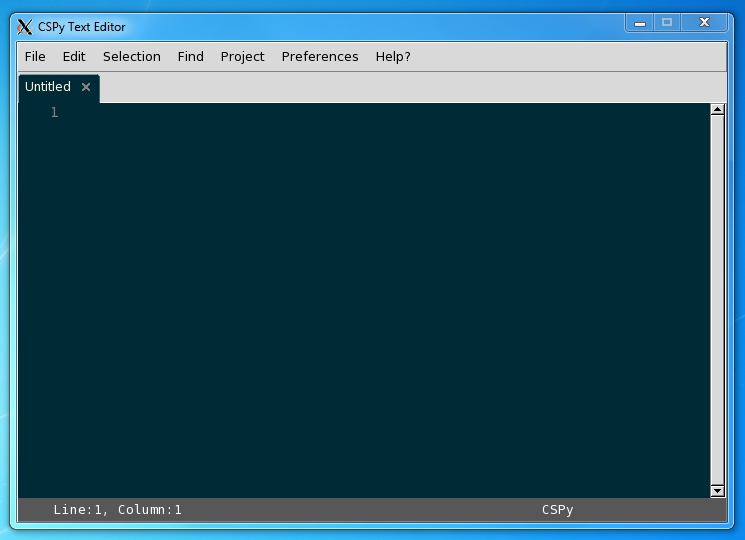
\includegraphics[width=\textwidth]{CSPyTextEditorMainScreen}
\captionof{figure}{This shows the program when it is initalized.}
\end{figure}

\begin{figure}[H]
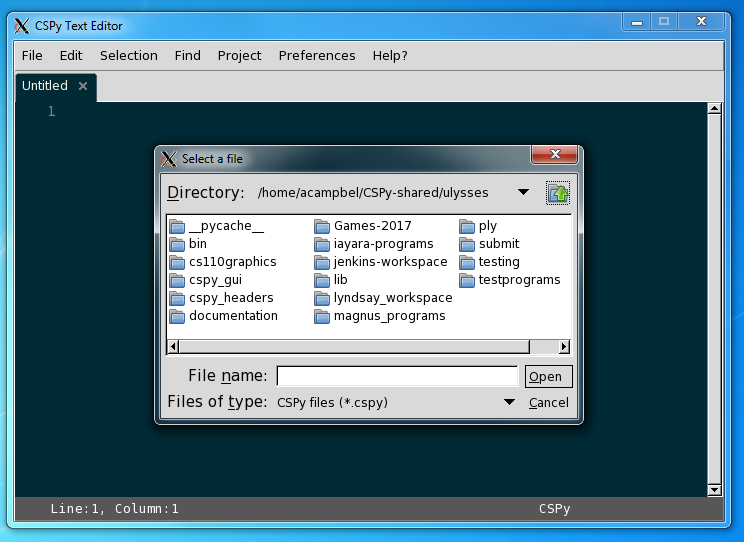
\includegraphics[width=\textwidth]{CSPyTextEditorOpenFile}
\captionof{figure}{This shows the program's open file prompt.}
\end{figure}

\begin{figure}[H]
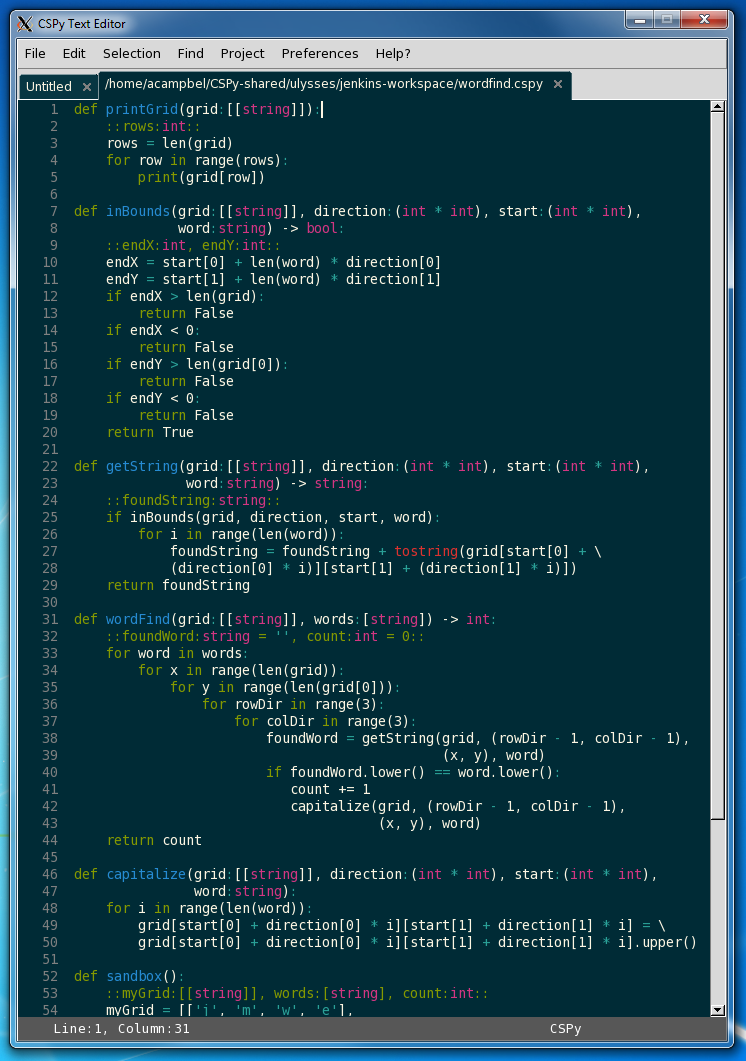
\includegraphics[width=\textwidth]{CSPyTextEditorSampleCode}
\captionof{figure}{This shows how the program highlights code and automatically numbers each line.}
\end{figure}

\begin{figure}[H]
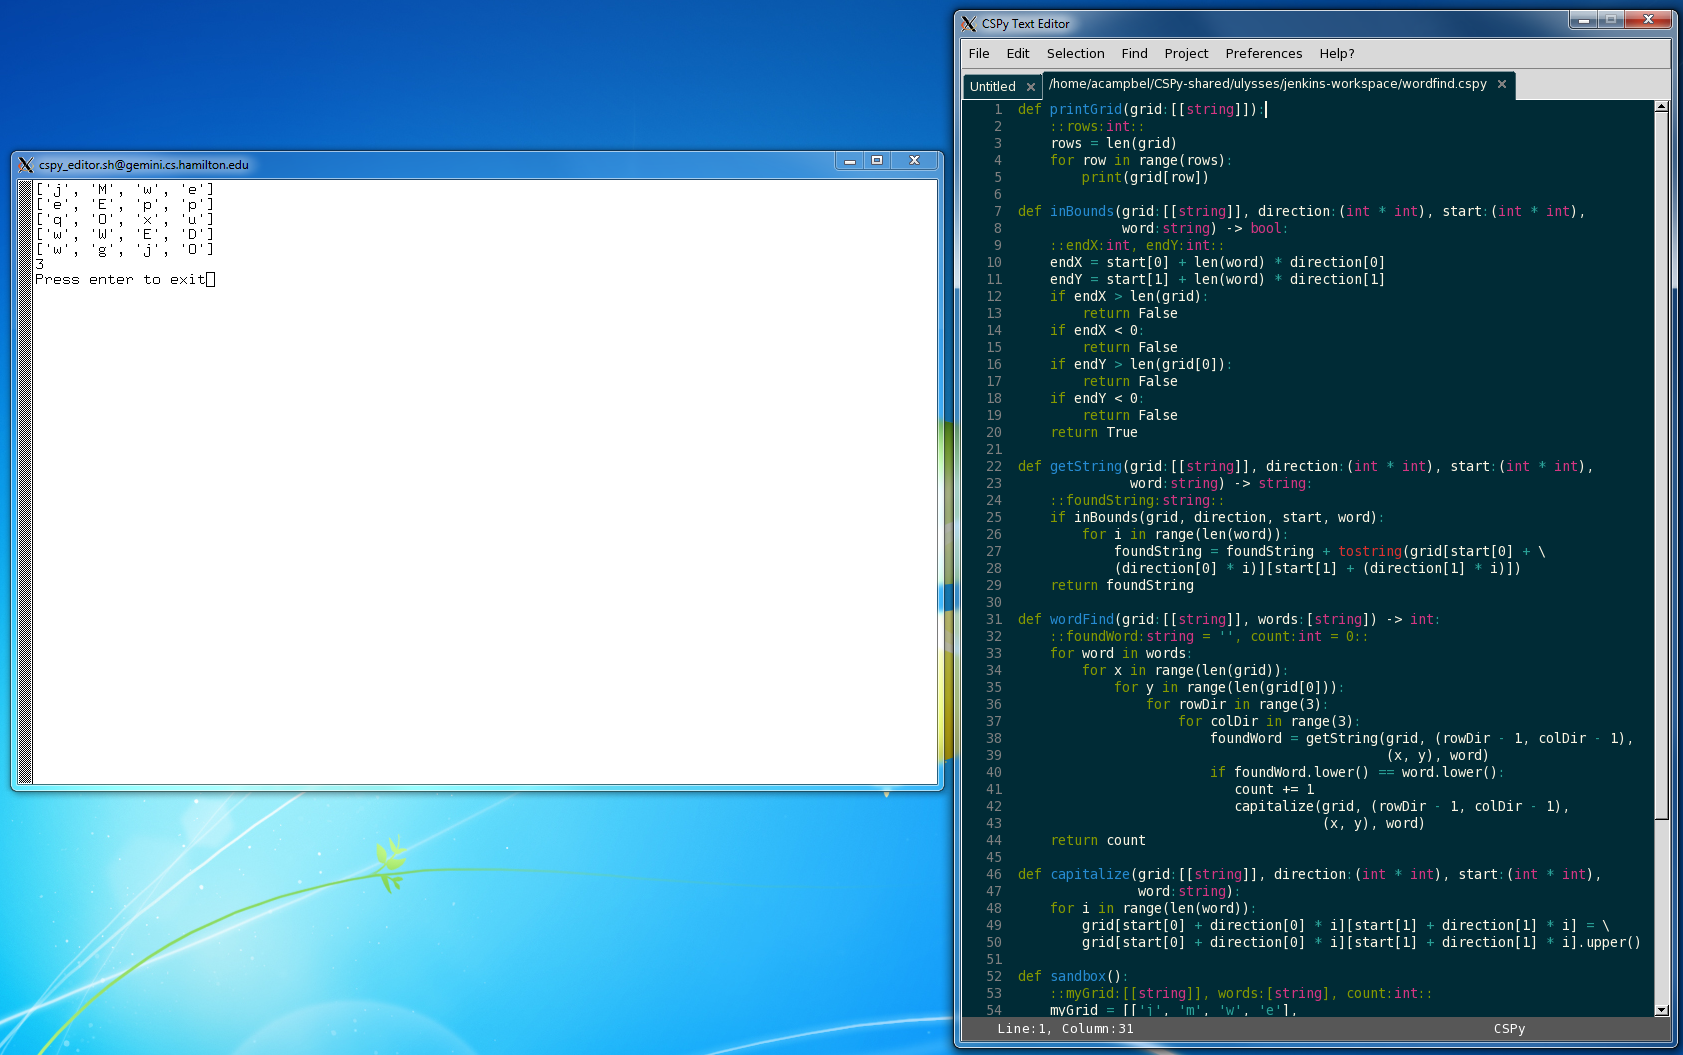
\includegraphics[width=\textwidth]{CSPyTextEditorSampleCodeWithOutput}
\captionof{figure}{This shows how the program runs files in a separate window.}
\end{figure}

\begin{figure}[H]
\centering
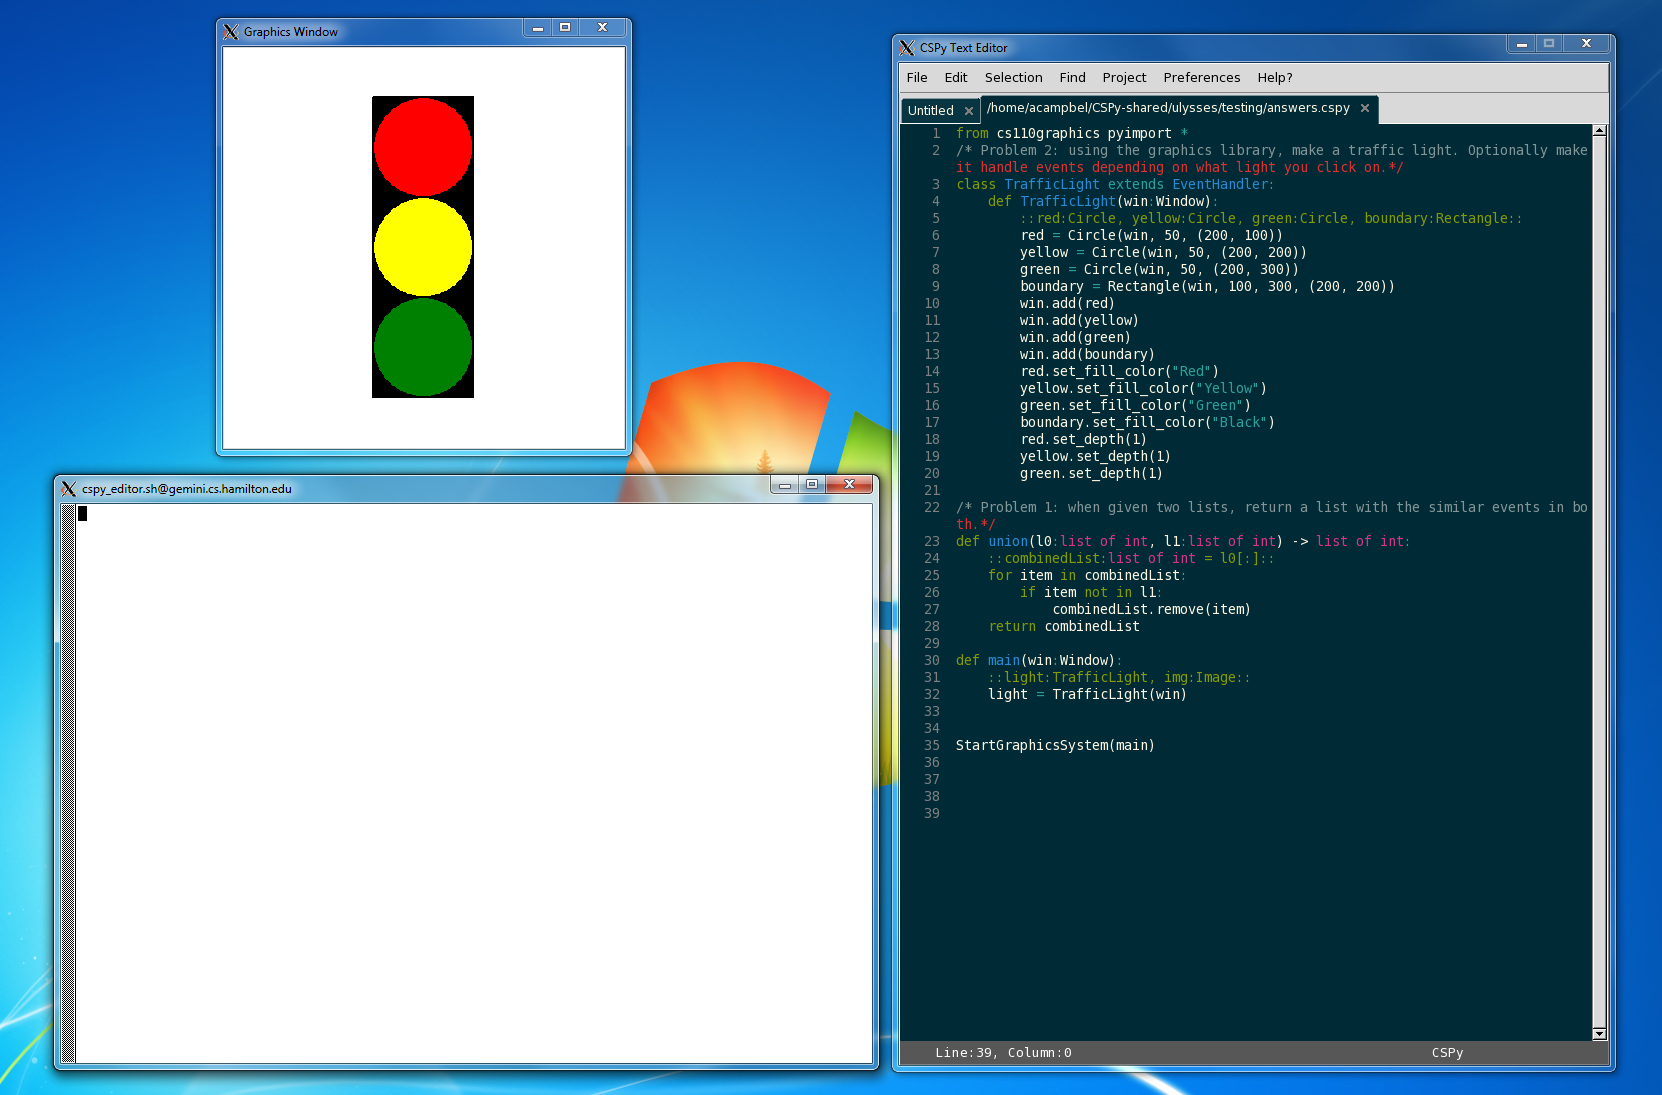
\includegraphics[width=\textwidth]{CSPyTextEditorSampleCodeWithGraphics}
\captionof{figure}{This shows how the program runs files in a separate window, and how it runs the graphics system in tandem.}
\end{figure}

\pagebreak

\section{CSPy Graphics Library Documentation}
\subsection{Introduction}
This section discusses the back end of the cs110graphics library, built predominantly by Matthew R. Jenkins '20, which is used in tandem with CSPy Text Editor to teach object oriented programming to beginning CS students. It is implemented in Tkinter, and is built off of a foundation by Professor Mark Bailey and subsequent improvements by Emily Sears and Kat Fuzesi in 2015.

\subsection{How The Frontend Works (From CSPy Ulysses Documentation For Teacher And Student Documentation)}

\subsubsection{The Basics}
To import the library, the line "\verb|from cs110graphics pyimport *|" needs to be the first line of your program. To put objects into the Graphics System, it requires a function which takes an object of type Window as a parameter.
\begin{verbatim}
    def function(win:Window):
\end{verbatim}
There are seven types of objects you can add to a window. Text, Image, Oval, Circle, Rectangle, Square, and Polygon. Each has its own method of initalization and requires specific parameters, but like the above function, each function requires a window object as the first parameter.

\begin{verbatim}
    def function(win:Window):
        ::circ:Circle::
        circ = Circle(win, 40, (200, 200))
        win.add(circ)
\end{verbatim}

To start the graphics system, instead of initalizing a function by calling it, you would wrap the function in a function called \verb|StartGraphicsSystem|. 
\begin{verbatim}
    def function(win:Window):
        ::circ:Circle::
        circ = Circle(win, 40, (200, 200))
        win.add(circ)

    StartGraphicsSystem(function)
\end{verbatim}

\begin{figure}[h!]

\includegraphics[width=.5\textwidth]{circle}
\centering
\captionof{figure}{The above code yields a circle of radius 40 in the center of the window.}
\end{figure}

The next page contains all of the graphical objects which are included in the graphics library, as well as sample code and implementations.

\pagebreak
\begin{itemize}
\item Text requires a string of text, but can optionally take a font size and a center. 
\begin{figure}[h!]
\centering
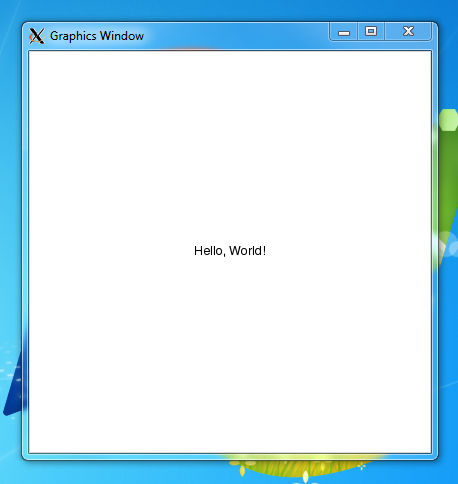
\includegraphics[width=.5\textwidth]{text}
\captionof{figure}{Text(win, "Hello, World!", 12, (200, 200))}
\end{figure}

\item Image requires a name of an image, which has to be in the current working directory. It can optionally take a width, a height, and a center. 
\begin{figure}[h!]
\centering

\includegraphics[width=.5\textwidth]{image}
\captionof{figure}{Image(win, "Lenna.png", 100, 100, (200, 200))}
\end{figure}

\pagebreak
\item Circles require a window, but can optionally take a radius and a center. 
\begin{figure}[h!]
\centering

\includegraphics[width=.5\textwidth]{circle}
\captionof{figure}{Circle(win, 40, (200, 200))}
\end{figure}

\item Ovals require a window, but can optionally take a radiusX, a radiusY, and a center. 
\begin{figure}[h!]
\centering

\includegraphics[width=.5\textwidth]{oval}
\captionof{figure}{Oval(win, 40, 60, (200, 200))} 
\end{figure}

\pagebreak

\item Squares require a window, but can optionally take a side length and a center. 
\begin{figure}[h!]
\centering

\includegraphics[width=.5\textwidth]{square}
\captionof{figure}{Square(win, 40, (200, 200))}
\end{figure}

\item Rectangles require a window, but can optionally take a width, a height, and a center. 
\begin{figure}[h!]
\centering
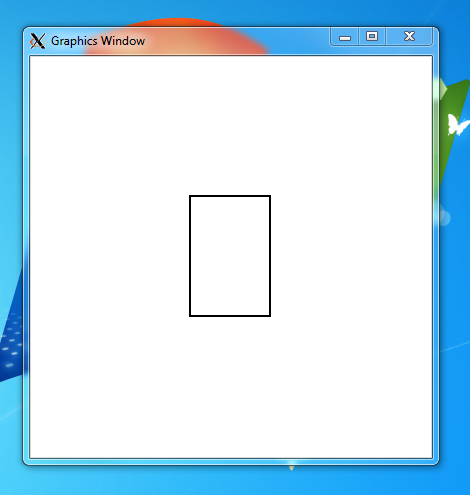
\includegraphics[width=.5\textwidth]{rectangle}
\captionof{figure}{Rectangle(win, 40, 60, (200, 200))}
\end{figure}

\pagebreak
\item Polygons require a window and a list of points. It cannot take anything optionally. 
\begin{figure}[h!]
\centering

\includegraphics[width=.5\textwidth]{polygon}
\captionof{figure}{Polygon(win, [(150, 150), (200, 236), (250, 150)])}
\end{figure}
\end{itemize}

\subsubsection{More Specific Methods}
Objects of type \verb|GraphicalObject| have access to \verb|GraphicalObject| methods, and Objects of type \verb|Fillable| have access to \verb|Fillable| methods, as well as \verb|GraphicalObject| methods. Some classes even have their own methods which can be accessed only by them.
\vskip.2in
\verb|GraphicalObjects| are all seven types of object that can be put on the canvas. They have the following methods accessible:

\begin{itemize}
\item \verb|add_handler(graphic:GraphicalObject)| - initalizes an EventHandler on the object and allows for overwriting of EventHandler functions by the class. (See Event Handling later in this section.)
\item \verb|get_center() -> tuple of (int * int)| - returns the center of the \verb|GraphicalObject|.
\item \verb|get_depth() -> int| - returns the depth of the \verb|GraphicalObject|.
\item \verb|move(dx:int, dy:int)| - Moves a \verb|GraphicalObject| dx pixels horizontally and dy pixels vertically.
\item \verb|move_to(point:tuple of (int * int))| - moves the center of a \verb|GraphicalObject| to the point.
\item \verb|set_depth(depth:int)| - sets the depth of the \verb|GraphicalObject|.
\end{itemize}
\vskip.2in
\verb|Fillables| are five of the objects that can be put on the canvas. They can have their fill colors and border colors changed, among other things. The \verb|Circle|, \verb|Oval|, \verb|Rectangle|, \verb|Square|, and \verb|Polygon| objects are all \verb|Fillables|.

\begin{itemize}
\item \verb|get_border_color() -> string| - returns the border color of a Fillable.
\item \verb|get_border_width() -> int| - returns the border width of a Fillable.
\item \verb|get_fill_color() -> string| - returns the fill color of a Fillable.
\item \verb|get_pivot() -> tuple of (int * int)| - returns the pivot point of a Fillable.
\item \verb|rotate(degrees:int)| - rotates a Fillable by degrees.
\item \verb|scale(factor:float)| - scales a Fillable's size by the scale factor. 
\item \verb|set_border_color(color:string)| - sets the border color of the Fillable.
\item \verb|set_border_width(width:int)| - sets the border width of the Fillable.
\item \verb|set_fill_color(color:string)| - sets the fill color of the Fillable.
\item \verb|set_pivot(pivot:tuple of (int * int))| - sets the pivot point of the Fillable.
\end{itemize}
You can either use names of colors like "\verb|yellow|", or you can use hexadecimal numbers in a string like "\verb|#FFFF00|" to set a color.

\begin{figure}[h]
\centering
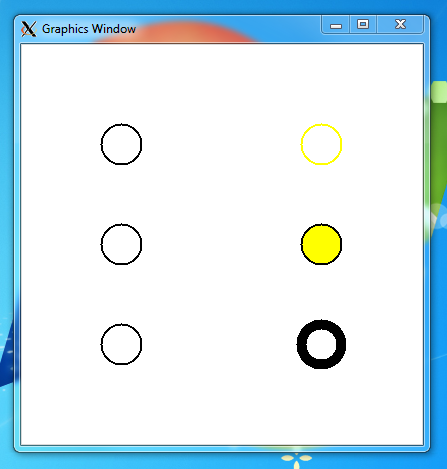
\includegraphics[width=.5\textwidth]{fillableAttributes}
\captionof{figure}{circ.set\_border\_color("yellow"), circ.set\_fill\_color("yellow"), circ.set\_border\_width(10)}


\end{figure}

Image methods (not including any inherited methods from GraphicalObject):
\begin{itemize}
\item \verb|resize(width:int, height:int)| - resizes an Image by width and height.
\item \verb|rotate(degrees:int)| - rotates an Image by degrees.
\item \verb|scale(factor:float)| - scales an Image's size by scale factor
\item \verb|size() -> tuple of (int * int)| - returns a tuple of the width and height of an Image.

\begin{figure}[h]
\centering
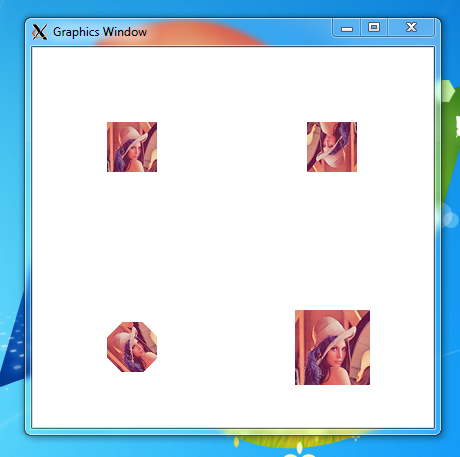
\includegraphics[width=.5\textwidth]{imageAttributes}
\captionof{figure}{img.rotate(180), img.rotate(45), img.scale(1.5)}
\end{figure}

\pagebreak

\end{itemize}
Text methods (not including any inherited methods from GraphicalObject):
\begin{itemize}
\item \verb|set_text(text:string)| - Sets the text of the Text object.
\item \verb|set_size(size:int)| - sets the point size of the Text object.
\end{itemize}
\vskip.1in
Circle methods (not including any inherited methods from GraphicalObject or Fillable):
\begin{itemize}
\item \verb|set_radius(radius:int)| - sets the radius of the Circle.
\end{itemize}
\vskip.1in
Oval methods (not including any inherited methods from GraphicalObject or Fillable):
\begin{itemize}
\item \verb|set_radii(radiusX:int, radiusY:int)| - sets the radii of the Oval.
\end{itemize}
\vskip.1in
Square methods (not including any inherited methods from GraphicalObject or Fillable):
\begin{itemize}
\item \verb|set_side_length(sideLength:int)| - sets the side length of the Square.
\end{itemize}
\vskip.1in
Rectangle methods (not including any inherited methods from GraphicalObject or Fillable):
\begin{itemize}
\item \verb|set_side_lengths(width:int, height:int)| - sets the width and height of the Rectangle. 
\end{itemize}

\subsubsection{Event Handling}
Event handling is the computer science term for sending keyboard and mouse commands to a graphical interface. The graphics library supports a rudimentary version of event handling.

There are two classes which do the work: \verb|Event|, and \verb|EventHandler|. \verb|Event| takes an keyboard or mouse event and converts it to a format which can be read by \verb|EventHandler|. In \verb|Event|, you can get the location where the event occurred, the mouse button that did it, the keyboard button that did it, or a description of the event. This is useful for handling different kinds of button input.
\vskip.1in
Below is a list of Event's methods:

\begin{itemize}
\item \verb|get_button() -> string| - returns the mouse button that generated the event. It will be one of the following:
\begin{itemize}
\item Left Mouse Button
\item Middle Mouse Button
\item Right Mouse Button
\end{itemize}
\item \verb|get_description() -> string| - returns the description of the event. It will be one of the following:
\begin{itemize}
\item Key Press
\item Key Release
\item Mouse Press
\item Mouse Release
\item Mouse Move
\item Mouse Enter
\item Mouse Leave
\end{itemize}
\item \verb|get_key() -> string| - returns the key that was pressed or released.
\item \verb|get_location() -> tuple of (int * int)| - returns the location of the mouse on the canvas.
\item \verb|get_root_location() -> tuple of (int * int)| - returns the location of the mouse on the monitor.
\end{itemize}

\verb|EventHandler| is a class which contains what is executed when an event is sent to specific objects. It is designed so that the user can overwrite the functions in the class and replace it with their own functions.
\vskip.1in
The functions that can be overwritten are as follows:
\begin{itemize}
\item \verb|handle_key_press(event:Event)| - handles a key press. 
\item \verb|handle_key_release(event:Event)| - handles a key release. 
\item \verb|handle_mouse_enter(event:Event)| - handles when the mouse enters an object. 
\item \verb|handle_mouse_leave(event:Event)| - handles when the mouse leaves an object. 
\item \verb|handle_mouse_move(event:Event)| - handles mouse movement. 
\item \verb|handle_mouse_press(event:Event)| - handles a mouse press. 
\item \verb|handle_mouse_release(event:Event)| - handles a mouse release. 
\end{itemize}

To overwrite, the user has to extend EventHandler and initalize it in their custom class:

\begin{verbatim}
class Button extends EventHandler:
    :: circ:Circle::
    def Button(win:Window):
        EventHandler.EventHandler()
        circ = Circle(win)
        win.add(circ)
        circ.add_handler(self)
\end{verbatim}

The user has defined a class called Button, which takes no parameters. The EventHandler is initalized, the Button's representation is made, and then the Button gets the ability to overload functions in EventHandler using the \verb|add_handler()| function.

To overwrite a function, all you have to do is define a function that matches the names of the functions you want to overwrite. If for example, the user wants the circle's color to change when they click on it, they would do this:

\begin{verbatim}
def handleMouseRelease(event:Event):
    circ.set_fill_color("yellow")
\end{verbatim}

After that is written by the user and run, the object's fill color will turn yellow when it is clicked. 

Each function requires an object of type Event to be attached so that if the user wants to know more details about the EventHandler, they can access the Event methods discussed above. For example, what if the user wants to know where the mouse was clicked within an object? The user would then use the Event class and call getMouseLocation() to find out:

\begin{verbatim}
def handleMouseRelease(event:Event):
    print(event.getMouseLocation())
\end{verbatim}

\subsubsection{Animations}

There are two ways to do animations. One is to use the Timer class. When initalized, a Timer takes a window, a delay (in milliseconds), and a function. The timer will re-run the function after each delay of time. To start the timer, call the \verb|start()| function. To stop the timer, call the \verb|stop()| function.

\begin{verbatim}
class Button:
    :: circ:Circle, timer:Timer, pressed:bool ::
    def Button(win:Window):
        circ = Circle(win)
        win.add(circ)
        timer = Timer(win, 200, flash)
        pressed = False
        timer.start()

    def flash():
        if pressed:
            circ.set_fill_color("")
            pressed = False
        else:
            circ.set_fill_color("yellow")
            pressed = True
\end{verbatim}

This code example has several parts to it. It first initalizes a Circle, a Timer and a Boolean. It creates the circle, adds it, creates the timer, sets the boolean to False, then starts the timer. The timer then runs the function \verb|flash|, which sets the fill color to yellow, then after 200 seconds sets it to be transparent.

Another way to do animations is to run an instance of the \verb|RunWithYieldDelay| class. This class takes a function which has the CSPy keyword \verb|yield| and then allows that function to run with a delay.

\begin{verbatim}
def main(win:Window):
    :: circ:Circle ::
    circ = Circle(win)
    win.add(circ)
    RunWithYieldDelay(win, move_circle(circ))

def move_circle(circ:Circle) -> generator of int:
    for i in range(10):
        circ.move(10, 0)
        yield 200
    raise StopIteration
\end{verbatim}

This function will keep running until the for loop stops.

\subsection{How The Backend Works}

Admittedly, it's very hard to describe the rationale behind certain design choices without leaving out details, but I'm going to try my best.

To start, I modeled my version of the graphics library to be very similar to Professor Bailey's and Emily Sears'. I did modify all of the functions behind it to fit to PEP8 style guidelines (for example, everything before was camelCase but now it's snake\_case). Consistency is something that we're trying to aim for with CSPy so I think following PEP8 guidelines is a good start to this.

The backend is built off TKinter. The Window object is where everything TKinter related lives, as it contains the Frame, the Canvas object, and a list of all objects. The list contains 3 elements: the object's depth, the object's tag, and the object itself. The tag is the alias of the object and any modifications such as tag binding are done to it.

When an object is made, it is created in its constructor (using TKinter's \verb|create_polygon| or \verb|create_image| or \verb|create_text| methods) and automatically added to the Window but it's marked as hidden/disabled. When the object is added to the Window using the \verb|Window.add()| method, it becomes visible and interactable. When it is removed using the \verb|Window.remove()|, it is removed from the canvas and the graphic list, the tag is set to none and the object is disabled.

Each object's constructor takes different formal parameters, but generally save to the same four attributes: a Window object, a width, a height, a center. From there the object generates a different polygon depending on its constructor: squares and rectangles generate 4 points, and then is added, but ovals and circles have a function \verb|_circle_gen| which generates a circle or oval. Each object is mutable after it is made, whether it be setting its dimensions or colors. Any change has to result in a tag change, because when an object is changed in most cases, a new object has to be made which is built off whatever change is requested (so if you want to rotate an oval 40 degrees, the oval has to have all of its points modified so that it's 40 degrees to the left, and then recreated and saved to that tag).

The Hierarchy is as follows:

\begin{figure}[ht!]
\centering
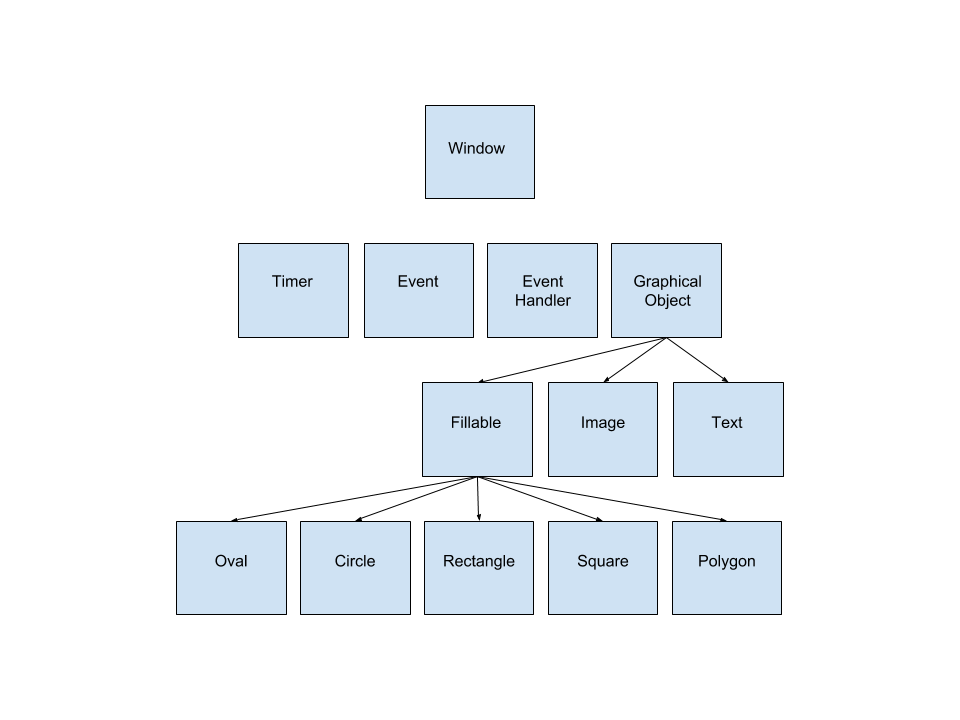
\includegraphics[width=\textwidth]{hierarchy}
\captionof{figure}{This is the basic hierarchy of the graphics library.}
\end{figure}

Functions like \verb|StartGraphicsSystem| and \verb|RunWithYieldDelay| are omitted from this hierarchy, as I wanted to show the relationship between each class with this diagram. 

EventHandling is bound on an object by object basis. Originally I thought that all of the keybinds had to be made as soon as the window was initalized and then they were overwritten by the user and their objects, but this ultimately ended up causing redundancies. The \verb|add_handler| function now does the binding. If it's a key based bind, it is added to the canvas, but if it's a mouse based bind, it is bound to the graphic. \verb|add_handler| passes the graphic's version of any EventHandler function to a function called \verb|call_handler|, which either adds an event if it's found in the function or omitted. 

Animations have both Timer and RunWithYieldDelay. Originally I thought by forcing the window to update (instead of using a mainloop) that RunWithYieldDelay would be rendered unnecessary, but it turns out that RunWithYieldDelay uses a different method of animation than I originally thought. It uses a generator, and at first I thought it would be too niche of an addition to the language, but I couldn't find any other way that wasn't either dangerous (like graphical threading) or impractical (like omitting the function altogether and encouraging the user to use the Timer class for all animations).

I like to think that my code is self documenting, and I tried my best to make it simple to read and simple to diagnose. If you're confused about anything, please feel free to email me at mjenkins@hamilton.edu.

\pagebreak

\section{Future Development Recommendations}
At the present moment, the only recommendations we can think of are improving CSPy and fixing any bugs we failed to notice, improving the graphics library by adding new functions and new features, and improving the design and implementation of the CSPy Text Editor.
\pagebreak
\section{Appendix 1: parser.out Grammar Rules}
cspy\_parser.py:
\begin{verbatim}
Rule 0     S' -> file
Rule 1     file -> optdoc importblock declaration_suite nonempty_block
Rule 2     file -> optdoc importblock declaration_suite empty
Rule 3     empty -> <empty>
Rule 4     optdoc -> DOCSTRING NL
Rule 5     optdoc -> empty
Rule 6     importblock -> nonempty_importblock
Rule 7     importblock -> empty
Rule 8     nonempty_importblock -> singleimport
Rule 9     singleimport -> import_statement
Rule 10    singleimport -> pyimport_statement
Rule 11    nonempty_importblock -> nonempty_importblock singleimport
Rule 12    import_statement -> IMPORT IDENTIFIER NL
Rule 13    import_statement -> IMPORT IDENTIFIER AS IDENTIFIER NL
Rule 14    import_statement -> FROM IDENTIFIER IMPORT TIMES NL
Rule 15    import_statement -> FROM IDENTIFIER IMPORT importlist NL
Rule 16    importlist -> IDENTIFIER
Rule 17    importlist -> IDENTIFIER AS IDENTIFIER
Rule 18    importlist -> importlist COMMA importlist
Rule 19    pyimport_statement -> PYIMPORT IDENTIFIER NL
Rule 20    pyimport_statement -> PYIMPORT IDENTIFIER AS IDENTIFIER NL
Rule 21    pyimport_statement -> FROM IDENTIFIER PYIMPORT TIMES NL
Rule 22    pyimport_statement -> FROM IDENTIFIER PYIMPORT importlist NL
Rule 23    declaration_suite -> variableblock classblock methodblock
Rule 24    declaration_suite -> PASS NL
Rule 25    variableblock -> COLONCOLON nonempty_variableblock COLONCOLON NL
Rule 26    variableblock -> empty empty
Rule 27    nonempty_variableblock -> declaration
Rule 28    nonempty_variableblock -> nonempty_variableblock COMMA nonempty_variableblock
Rule 29    declaration -> IDENTIFIER COLON type
Rule 30    declaration -> IDENTIFIER COLON type EQUALS expression
Rule 31    classblock -> class_definition classblock
Rule 32    classblock -> empty
Rule 33    class_definition -> CLASS IDENTIFIER opt_extends COLON NL INDENT class_suite DEDENT
Rule 34    class_suite -> optdoc declaration_suite
Rule 35    opt_extends -> EXTENDS type
Rule 36    opt_extends -> empty empty
Rule 37    methodblock -> subroutine_definition methodblock
Rule 38    methodblock -> empty
Rule 39    subroutine_definition -> function_definition
Rule 40    subroutine_definition -> procedure_definition
Rule 41    function_definition -> DEF IDENTIFIER LPAREN argumentlist RPAREN ARROW type COLON suite
Rule 42    procedure_definition -> DEF IDENTIFIER LPAREN argumentlist RPAREN COLON suite
Rule 43    argumentlist -> nonempty_argumentlist COMMA nonempty_defaultlist
Rule 44    argumentlist -> nonempty_argumentlist empty empty
Rule 45    argumentlist -> empty empty empty
Rule 46    argumentlist -> nonempty_defaultlist empty empty
Rule 47    nonempty_argumentlist -> IDENTIFIER COLON type
Rule 48    nonempty_argumentlist -> nonempty_argumentlist COMMA nonempty_argumentlist
Rule 49    nonempty_defaultlist -> nonempty_defaultlist COMMA nonempty_defaultlist
Rule 50    nonempty_defaultlist -> IDENTIFIER COLON type EQUALS expression
Rule 51    suite -> NL INDENT optdoc block DEDENT
Rule 52    suite -> statement_simple NL
Rule 53    block -> variableblock nonempty_block
Rule 54    nonempty_block -> statement_complex empty
Rule 55    nonempty_block -> statement_complex nonempty_block
Rule 56    statement_complex -> loop
Rule 57    statement_complex -> conditional
Rule 58    statement_complex -> try_except
Rule 59    statement_complex -> statement_multi NL
Rule 60    statement_complex -> statement_multi SEMICOLON NL
Rule 61    statement_multi -> statement_multi SEMICOLON statement_simple
Rule 62    statement_multi -> statement_simple
Rule 63    statement_simple -> assignment
Rule 64    statement_simple -> procedure_call
Rule 65    statement_simple -> return
Rule 66    statement_simple -> assert
Rule 67    statement_simple -> yield
Rule 68    statement_simple -> CONTINUE
Rule 69    statement_simple -> BREAK
Rule 70    statement_simple -> PASS
Rule 71    statement_simple -> raise
Rule 72    statement_simple -> delete
Rule 73    raise -> RAISE IDENTIFIER
Rule 74    raise -> RAISE function_call
Rule 75    raise -> RAISE empty
Rule 76    delete -> DEL expression
Rule 77    loop -> while_loop
Rule 78    loop -> for_loop
Rule 79    while_loop -> WHILE expression COLON suite
Rule 80    for_loop -> FOR IDENTIFIER IN expression COLON suite
Rule 81    for_loop -> FOR IDENTIFIER IN expression DOTDOT expression COLON suite
Rule 82    conditional -> IF expression COLON suite conditional_extension
Rule 83    conditional_extension -> empty
Rule 84    conditional_extension -> ELIF expression COLON suite conditional_extension
Rule 85    conditional_extension -> ELSE COLON suite
Rule 86    try_except -> TRY COLON suite exceptlist_nonempty empty empty
Rule 87    try_except -> TRY COLON suite exceptlist_nonempty except_else empty
Rule 88    try_except -> TRY COLON suite exceptlist_nonempty empty except_finally
Rule 89    try_except -> TRY COLON suite exceptlist_nonempty except_else except_finally
Rule 90    try_except -> TRY COLON suite empty empty except_finally
Rule 91    except_simple -> EXCEPT COLON suite
Rule 92    except_alias -> EXCEPT IDENTIFIER AS IDENTIFIER COLON suite exceptlist
Rule 93    except_specific -> EXCEPT IDENTIFIER COLON suite exceptlist
Rule 94    except_else -> ELSE COLON suite
Rule 95    except_finally -> FINALLY COLON suite
Rule 96    exceptlist_nonempty -> except_simple
Rule 97    exceptlist_nonempty -> except_alias
Rule 98    exceptlist_nonempty -> except_specific
Rule 99    exceptlist -> except_simple
Rule 100   exceptlist -> except_alias
Rule 101   exceptlist -> except_specific
Rule 102   exceptlist -> empty
Rule 103   assignment -> indexing assignment_operator expression
Rule 104   assignment -> slicing assignment_operator expression
Rule 105   assignment -> variable assignment_operator expression
Rule 106   assignment -> member assignment_operator expression
Rule 107   assignment_operator -> EQUALS
Rule 108   assignment_operator -> PLUSEQU
Rule 109   assignment_operator -> MINUSEQU
Rule 110   assignment_operator -> TIMESEQU
Rule 111   assignment_operator -> DIVEQU
Rule 112   assignment_operator -> MODEQU
Rule 113   assignment_operator -> BITANDEQU
Rule 114   assignment_operator -> BITOREQU
Rule 115   assignment_operator -> BITXOREQU
Rule 116   assignment_operator -> LSHIFTEQU
Rule 117   assignment_operator -> RSHIFTEQU
Rule 118   assignment_operator -> POWEQU
Rule 119   assignment_operator -> INTDIVEQU
Rule 120   indexing -> expression LBRACKET expression RBRACKET
Rule 121   slicing -> expression LBRACKET expression COLON expression optslice RBRACKET
Rule 122   slicing -> expression LBRACKET empty COLON expression optslice RBRACKET
Rule 123   slicing -> expression LBRACKET expression COLON empty optslice RBRACKET
Rule 124   slicing -> expression LBRACKET empty COLON empty optslice RBRACKET
Rule 125   optslice -> empty empty
Rule 126   optslice -> COLON empty
Rule 127   optslice -> COLON expression
Rule 128   procedure_call -> expression LPAREN expressionlist RPAREN
Rule 129   return -> RETURN empty
Rule 130   return -> RETURN expression
Rule 131   assert -> assertnomessage
Rule 132   assert -> assertmessage
Rule 133   assertnomessage -> ASSERT expression
Rule 134   assertmessage -> ASSERT expression COMMA literal
Rule 135   yield -> YIELD expression
Rule 136   type -> function_type
Rule 137   type -> procedure_type
Rule 138   type -> tuple_type
Rule 139   type -> list_type
Rule 140   type -> dictionary_type
Rule 141   type -> set_type
Rule 142   type -> frozenset_type
Rule 143   type -> generator_type
Rule 144   type -> member_type
Rule 145   type -> IDENTIFIER
Rule 146   member_type -> IDENTIFIER DOT IDENTIFIER
Rule 147   generator_type -> GENERATOR OF type
Rule 148   function_type -> FN LPAREN typelist RPAREN ARROW type
Rule 149   procedure_type -> PROC LPAREN typelist RPAREN
Rule 150   typelist -> nonempty_typelist COMMA nonempty_default_typelist
Rule 151   typelist -> nonempty_typelist empty empty
Rule 152   typelist -> empty empty nonempty_default_typelist
Rule 153   typelist -> empty empty empty
Rule 154   nonempty_typelist -> type
Rule 155   nonempty_typelist -> nonempty_typelist COMMA nonempty_typelist
Rule 156   nonempty_default_typelist -> QMARK type
Rule 157   nonempty_default_typelist -> nonempty_default_typelist COMMA nonempty_default_typelist
Rule 158   tuple_type -> tupleof
Rule 159   tuple_type -> tupleparens
Rule 160   tupleof -> TUPLE OF LPAREN tuple_typelist RPAREN
Rule 161   tupleparens -> LPAREN tuple_typelist RPAREN
Rule 162   tuple_typelist -> nonempty_tuple_typelist
Rule 163   tuple_typelist -> empty
Rule 164   nonempty_tuple_typelist -> type
Rule 165   nonempty_tuple_typelist -> nonempty_tuple_typelist TIMES nonempty_tuple_typelist
Rule 166   list_type -> listof
Rule 167   list_type -> listbracket
Rule 168   listof -> LIST OF type
Rule 169   listbracket -> LBRACKET type RBRACKET
Rule 170   set_type -> SET OF type
Rule 171   frozenset_type -> FROZENSET OF type
Rule 172   dictionary_type -> DICT OF LBRACKET type BITOR type RBRACKET
Rule 173   expression -> calculation
Rule 174   expression -> function_call
Rule 175   expression -> grouping
Rule 176   expression -> literal
Rule 177   expression -> indexing
Rule 178   expression -> slicing
Rule 179   expression -> ternary
Rule 180   expression -> member
Rule 181   expression -> identity
Rule 182   expression -> membership
Rule 183   expression -> variable
Rule 184   calculation -> expression PLUS expression
Rule 185   calculation -> expression MINUS expression
Rule 186   calculation -> expression TIMES expression
Rule 187   calculation -> expression DIVIDE expression
Rule 188   calculation -> expression PERCENT expression
Rule 189   calculation -> expression INTDIV expression
Rule 190   calculation -> expression POW expression
Rule 191   calculation -> expression BITOR expression
Rule 192   calculation -> expression BITAND expression
Rule 193   calculation -> expression LSHIFT expression
Rule 194   calculation -> expression RSHIFT expression
Rule 195   calculation -> expression EQUALTO expression
Rule 196   calculation -> expression NEQUALTO expression
Rule 197   calculation -> expression LT expression
Rule 198   calculation -> expression LE expression
Rule 199   calculation -> expression GT expression
Rule 200   calculation -> expression GE expression
Rule 201   calculation -> expression REQUALTO expression
Rule 202   calculation -> expression BOOLOR expression
Rule 203   calculation -> expression BOOLAND expression
Rule 204   calculation -> expression OR expression
Rule 205   calculation -> expression AND expression
Rule 206   calculation -> expression CARET expression
Rule 207   expression -> MINUS expression
Rule 208   expression -> PLUS expression
Rule 209   expression -> TILDE expression
Rule 210   expression -> EXMARK expression
Rule 211   expression -> NOT expression
Rule 212   function_call -> expression LPAREN expressionlist RPAREN
Rule 213   expressionlist -> nonempty_expressionlist
Rule 214   expressionlist -> empty
Rule 215   nonempty_expressionlist -> expression
Rule 216   nonempty_expressionlist -> nonempty_expressionlist COMMA nonempty_expressionlist
Rule 217   grouping -> LPAREN expression RPAREN
Rule 218   literal -> INTLITERAL
Rule 219   literal -> FLOATLITERAL
Rule 220   literal -> BOOLLITERAL
Rule 221   literal -> STRINGLITERAL
Rule 222   literal -> DOCSTRING
Rule 223   literal -> NONE
Rule 224   literal -> function_literal
Rule 225   literal -> procedure_literal
Rule 226   literal -> tuple_literal
Rule 227   literal -> list_literal
Rule 228   literal -> dictionary_literal
Rule 229   literal -> set_literal
Rule 230   function_literal -> LAMBDA LPAREN argumentlist RPAREN ARROW type COLON LPAREN expression RPAREN
Rule 231   tuple_literal -> LPAREN tuplelist RPAREN
Rule 232   tuplelist -> nonempty_tuple
Rule 233   tuplelist -> empty
Rule 234   nonempty_tuple -> singletontuple
Rule 235   nonempty_tuple -> crosstuple
Rule 236   singletontuple -> nonempty_expressionlist COMMA
Rule 237   crosstuple -> nonempty_expressionlist
Rule 238   list_literal -> LBRACKET expressionlist RBRACKET
Rule 239   dictionary_literal -> LCURLY dictionarylist RCURLY
Rule 240   dictionarylist -> nonempty_dictionarylist
Rule 241   dictionarylist -> empty
Rule 242   nonempty_dictionarylist -> expression COLON expression
Rule 243   nonempty_dictionarylist -> nonempty_dictionarylist COMMA nonempty_dictionarylist
Rule 244   set_literal -> LCURLY nonempty_expressionlist RCURLY
Rule 245   variable -> IDENTIFIER
Rule 246   ternary -> expression QMARK expression COLON expression
Rule 247   member -> expression DOT IDENTIFIER
Rule 248   identity -> expression IS expression
Rule 249   identity -> expression ISNOT expression
Rule 250   membership -> expression IN expression
Rule 251   membership -> expression NOTIN expression
Rule 252   variableblock -> COLONCOLON error COLONCOLON NL
Rule 253   declaration -> IDENTIFIER COLON error EQUALS expression
Rule 254   class_definition -> CLASS IDENTIFIER opt_generic opt_extends error NL INDENT class_suite DEDENT
Rule 255   class_definition -> CLASS IDENTIFIER opt_generic opt_extends COLON NL INDENT error DEDENT
Rule 256   opt_generic -> LT error GT
Rule 257   function_definition -> DEF error LPAREN argumentlist RPAREN ARROW type COLON suite
Rule 258   function_definition -> DEF IDENTIFIER LPAREN argumentlist error ARROW type COLON suite
Rule 259   function_definition -> DEF IDENTIFIER LPAREN argumentlist RPAREN ARROW error COLON suite
Rule 260   procedure_definition -> DEF error LPAREN argumentlist RPAREN COLON suite
Rule 261   procedure_definition -> DEF IDENTIFIER LPAREN argumentlist error COLON suite
Rule 262   nonempty_argumentlist -> error COLON type
Rule 263   nonempty_defaultlist -> IDENTIFIER COLON error EQUALS expression
Rule 264   while_loop -> WHILE error COLON suite
Rule 265   for_loop -> FOR error IN expression COLON suite
Rule 266   for_loop -> FOR IDENTIFIER IN error COLON suite
Rule 267   for_loop -> FOR error IN expression DOTDOT expression COLON suite
Rule 268   for_loop -> FOR IDENTIFIER IN error DOTDOT expression COLON suite
Rule 269   for_loop -> FOR IDENTIFIER IN expression DOTDOT error COLON suite
Rule 270   conditional -> IF error COLON suite conditional_extension
Rule 271   conditional_extension -> ELIF error COLON suite conditional_extension
Rule 272   except_alias -> EXCEPT error AS IDENTIFIER COLON suite exceptlist
Rule 273   except_alias -> EXCEPT IDENTIFIER AS error COLON suite exceptlist
Rule 274   except_specific -> EXCEPT error COLON suite exceptlist
Rule 275   indexing -> expression LBRACKET error RBRACKET
Rule 276   slicing -> expression LBRACKET error COLON expression optslice RBRACKET
Rule 277   slicing -> expression LBRACKET expression COLON expression error RBRACKET
Rule 278   procedure_call -> expression LPAREN error RPAREN
Rule 279   function_type -> FN LPAREN error RPAREN ARROW type
Rule 280   procedure_type -> PROC LPAREN error RPAREN
Rule 281   dictionary_type -> DICT error LBRACKET type BITOR type RBRACKET
Rule 282   dictionary_type -> DICT OF LBRACKET error BITOR type RBRACKET
Rule 283   dictionary_type -> DICT OF LBRACKET type BITOR error RBRACKET
Rule 284   tuple_type -> TUPLE error LPAREN tuple_typelist RPAREN
Rule 285   tuple_type -> TUPLE OF LPAREN error RPAREN
Rule 286   function_literal -> LAMBDA LPAREN error RPAREN ARROW type COLON LPAREN expression RPAREN
Rule 287   function_literal -> LAMBDA LPAREN argumentlist RPAREN ARROW error COLON LPAREN expression RPAREN
Rule 288   function_literal -> LAMBDA LPAREN argumentlist RPAREN ARROW type COLON LPAREN error RPAREN
Rule 289   procedure_literal -> LAMBDA LPAREN error RPAREN COLON LPAREN statement_simple RPAREN
Rule 290   procedure_literal -> LAMBDA LPAREN argumentlist RPAREN error LPAREN statement_simple RPAREN
Rule 291   procedure_literal -> LAMBDA LPAREN argumentlist RPAREN COLON LPAREN error RPAREN
Rule 292   list_literal -> LBRACKET error RBRACKET
Rule 293   dictionary_literal -> LCURLY error RCURLY
\end{verbatim}
\pagebreak
\noindent \verb|cspy\_header\_parser.py|:
\begin{verbatim}
Rule 0     S' -> file
Rule 1     file -> optdoc importblock declaration_suite
Rule 2     empty -> <empty>
Rule 3     optdoc -> DOCSTRING NL
Rule 4     optdoc -> empty
Rule 5     importblock -> nonempty_importblock
Rule 6     importblock -> empty
Rule 7     nonempty_importblock -> singleimport
Rule 8     singleimport -> pyimport_statement
Rule 9     nonempty_importblock -> nonempty_importblock singleimport
Rule 10    pyimport_statement -> PYIMPORT IDENTIFIER NL
Rule 11    pyimport_statement -> PYIMPORT IDENTIFIER AS IDENTIFIER NL
Rule 12    pyimport_statement -> FROM IDENTIFIER PYIMPORT TIMES NL
Rule 13    pyimport_statement -> FROM IDENTIFIER PYIMPORT importlist NL
Rule 14    importlist -> IDENTIFIER
Rule 15    importlist -> IDENTIFIER AS IDENTIFIER
Rule 16    importlist -> importlist COMMA importlist
Rule 17    declaration_suite -> variableblock classblock methodblock
Rule 18    variableblock -> COLONCOLON nonempty_variableblock COLONCOLON NL
Rule 19    variableblock -> empty empty
Rule 20    nonempty_variableblock -> declaration
Rule 21    nonempty_variableblock -> nonempty_variableblock COMMA nonempty_variableblock
Rule 22    declaration -> IDENTIFIER COLON type
Rule 23    classblock -> class_definition classblock
Rule 24    classblock -> empty
Rule 25    class_definition -> CLASS IDENTIFIER opt_extends COLON NL INDENT class_suite DEDENT
Rule 26    class_suite -> optdoc declaration_suite
Rule 27    opt_extends -> EXTENDS type
Rule 28    opt_extends -> empty empty
Rule 29    methodblock -> subroutine_definition methodblock
Rule 30    methodblock -> empty
Rule 31    subroutine_definition -> function_definition
Rule 32    subroutine_definition -> procedure_definition
Rule 33    function_definition -> DEF IDENTIFIER LPAREN argumentlist RPAREN ARROW type NL
Rule 34    procedure_definition -> DEF IDENTIFIER LPAREN argumentlist RPAREN NL
Rule 35    argumentlist -> nonempty_argumentlist COMMA nonempty_defaultlist
Rule 36    argumentlist -> nonempty_argumentlist empty empty
Rule 37    argumentlist -> empty empty empty
Rule 38    argumentlist -> nonempty_defaultlist empty empty
Rule 39    nonempty_argumentlist -> IDENTIFIER COLON type
Rule 40    nonempty_argumentlist -> nonempty_argumentlist COMMA nonempty_argumentlist
Rule 41    nonempty_defaultlist -> nonempty_defaultlist COMMA nonempty_defaultlist
Rule 42    nonempty_defaultlist -> IDENTIFIER COLON QMARK type
Rule 43    type -> function_type
Rule 44    type -> procedure_type
Rule 45    type -> tuple_type
Rule 46    type -> list_type
Rule 47    type -> dictionary_type
Rule 48    type -> set_type
Rule 49    type -> frozenset_type
Rule 50    type -> generator_type
Rule 51    type -> IDENTIFIER
Rule 52    function_type -> FN LPAREN typelist RPAREN ARROW type
Rule 53    procedure_type -> PROC LPAREN typelist RPAREN
Rule 54    typelist -> nonempty_typelist COMMA nonempty_default_typelist
Rule 55    typelist -> nonempty_typelist empty empty
Rule 56    typelist -> empty empty nonempty_default_typelist
Rule 57    typelist -> empty empty empty
Rule 58    nonempty_typelist -> type
Rule 59    nonempty_typelist -> nonempty_typelist COMMA nonempty_typelist
Rule 60    nonempty_default_typelist -> QMARK type
Rule 61    nonempty_default_typelist -> nonempty_default_typelist COMMA nonempty_default_typelist
Rule 62    tuple_type -> tupleof
Rule 63    tuple_type -> tupleparens
Rule 64    tupleof -> TUPLE OF LPAREN tuple_typelist RPAREN
Rule 65    tupleparens -> LPAREN tuple_typelist RPAREN
Rule 66    tuple_typelist -> nonempty_tuple_typelist
Rule 67    tuple_typelist -> empty
Rule 68    nonempty_tuple_typelist -> type
Rule 69    nonempty_tuple_typelist -> nonempty_tuple_typelist TIMES nonempty_tuple_typelist
Rule 70    list_type -> listof
Rule 71    list_type -> listbracket
Rule 72    listof -> LIST OF type
Rule 73    listbracket -> LBRACKET type RBRACKET
Rule 74    set_type -> SET OF type
Rule 75    frozenset_type -> FROZENSET OF type
Rule 76    generator_type -> GENERATOR OF type
Rule 77    dictionary_type -> DICT OF LBRACKET type BITOR type RBRACKET
Rule 78    variableblock -> COLONCOLON error COLONCOLON NL
Rule 79    class_definition -> CLASS IDENTIFIER opt_extends error NL INDENT class_suite DEDENT
Rule 80    class_definition -> CLASS IDENTIFIER opt_extends COLON NL INDENT error DEDENT
Rule 81    function_definition -> DEF error LPAREN argumentlist RPAREN ARROW type
Rule 82    function_definition -> DEF IDENTIFIER LPAREN argumentlist error ARROW type
Rule 83    function_definition -> DEF IDENTIFIER LPAREN argumentlist RPAREN ARROW error
Rule 84    procedure_definition -> DEF error LPAREN argumentlist RPAREN
Rule 85    procedure_definition -> DEF IDENTIFIER LPAREN argumentlist error
Rule 86    nonempty_argumentlist -> error COLON type
Rule 87    function_type -> FN LPAREN error RPAREN ARROW type
Rule 88    procedure_type -> PROC LPAREN error RPAREN
Rule 89    dictionary_type -> DICT error LBRACKET type BITOR type RBRACKET
Rule 90    dictionary_type -> DICT OF LBRACKET error BITOR type RBRACKET
Rule 91    dictionary_type -> DICT OF LBRACKET type BITOR error RBRACKET
\end{verbatim}
\pagebreak
\section{Appendix 2: Types}
\textbf{Int:} A numeric type.\\
Binary Operators:\\
\begin{tabular}{|c|c|}
\hline
Addition & \verb|+| \\
\hline
Subtraction & \verb|-| \\
\hline
Multiplication & \verb|*| \\
\hline
Division & \verb|/| \\
\hline
Floor Division & \verb|//| \\
\hline
Exponentiation & \verb|**| \\
\hline
Modulus & \verb|%| \\
\hline
Bitwise And & \verb|&| \\
\hline
Bitwise Or & \verb!|! \\
\hline
Bitwise Xor & \verb|^| \\
\hline
Bitwise Invert & \verb|~| \\
\hline
Equals & \verb|==| \\
\hline
Not Equals & \verb|!=| \\
\hline
Greater Than & \verb|>| \\
\hline
Less Than & \verb|<| \\
\hline
Greater Or Equal To & \verb|>=| \\
\hline
Less Or Equal To & \verb|<=| \\ 
\hline
Bitwise Left Shift & \verb|<<| \\
\hline
Bitwise Right Shift & \verb|>>| \\
\hline
\end{tabular}
\vskip.2in
Unary Operators:\\
\begin{tabular}{|c|c|}
\hline
Positive & + \\
\hline
Negative & - \\
\hline
\end{tabular}
\vskip.2in
Type Conversion:
\begin{itemize}
\item Float via the \verb|tofloat| built in function
\item String via the \verb|tostring| or \verb|repr| built in function
\end{itemize}
Additional Operations:
\begin{itemize}
\item Supports augmented assignment.
\end{itemize}
\vskip.2in

\textbf{Float:} A numeric type.
\vskip.1in
Binary Operators: \\
\begin{tabular}{|c|c|}
\hline
Addition & \verb|+| \\
\hline
Subtraction & \verb|-| \\
\hline
Multiplication & \verb|*| \\
\hline
Division & \verb|/| \\
\hline
Floor Division & \verb|//| \\
\hline
Exponentiation & \verb|**| \\
\hline
Modulus & \verb|%| \\
\hline
Equals & \verb|==| \\
\hline
Not Equals & \verb|!=| \\
\hline
Greater Than & \verb|>| \\
\hline
Less Than & \verb|<| \\
\hline
Greater Or Equal To & \verb|>=| \\
\hline
Less Or Equal To & \verb|<=| \\ 
\hline
\end{tabular}
\vskip.2in
Unary Operators:\\
\begin{tabular}{|c|c|}
\hline
Positive & + \\
\hline
Negative & - \\
\hline
\end{tabular}
\vskip.2in
Type Conversion:
\begin{itemize}
\item Int via the \verb|toint| or \verb|round| built in function
\item String via the \verb|tostring| or \verb|repr| built in function
\end{itemize}
Additional Operations:
\begin{itemize}
\item Supports augmented assignment.
\end{itemize}
\vskip.2in

\textbf{Bool:} \\
Binary Operators: \\
\begin{tabular}{|c|c|}
\hline
Boolean And & \verb|and| \\
\hline
Boolean And & \verb|&&| \\
\hline
Boolean Or & \verb|or| \\
\hline
Boolean Or & \verb!||! \\
\hline
\end{tabular}
\vskip.2in
Unary Operators:\\
\begin{tabular}{|c|c|}
\hline
Boolean Not & \verb|not| \\
\hline
\end{tabular}
\vskip.2in
Type Conversion:
\begin{itemize}
\item String via the \verb|tostring| or \verb|repr| built in function
\end{itemize}
(NOTE: In Python, bool is a subclass of Integer, therefore Integer binary operators such as '+', '-', etc. would be applicable to Boolean values as well. This is not the case in CSPy, as there is no benefit for a beginner programmer to use any of these operators on boolean.) \\
\vskip.2in
\textbf{String:} A sequence type.
\vskip.1in
Binary Operators: \\
\begin{tabular}{|c|c|}
\hline
Concatenate & \verb|+| \\
\hline
Repetition & \verb|*| \\
\hline
Greater Than & \verb|>| \\
\hline
Less Than & \verb|<| \\
\hline
Greater Or Equal To & \verb|>=| \\
\hline
Less Or Equal To & \verb|<=| \\ 
\hline
Equals & \verb|==| \\
\hline
Not Equals & \verb|!=| \\ 
\hline
\end{tabular}
\vskip.2in
Type Conversion:
\begin{itemize}
\item Integer via \verb|toint| built-in function 
\item Float via \verb|tofloat| built-in function
\item List, Set, or Frozenset via \verb|tolist| or \verb|makeset| or \verb|frzset| built-in functions
\end{itemize}
Additional Operations:
\begin{itemize}
\item String supports indexing, slicing, membership, iterations, and use of the \verb|len()| function. Also supports augmented assignment. 
\end{itemize}

\vskip.2in
\textbf{List:} A sequence type.
\vskip.1in
Binary Operators: \\
\begin{tabular}{|c|c|}
\hline
Concatenate & \verb|+| \\
\hline
Repetition & \verb|*| \\
\hline
Equals & \verb|==| \\
\hline
Not Equals & \verb|!=| \\ 
\hline
\end{tabular}
\vskip.2in
Type Conversion:
\begin{itemize}
\item String via \verb|tostring| or \verb|repr| built-in function
\item Set or Frozenset via \verb|makeset| or \verb|frzset| built-in functions
\item Bool via \verb|tobool| built-in function
\end{itemize}
Additional Operations:
\begin{itemize}
\item List supports indexing, slicing, membership, iterations, and use of the \verb|len()| function. Also supports augmented assignment. 
\end{itemize}
\vskip.2in

\textbf{Tuples:} A sequence type.
Tuples are heterogeneous, and can contain elements of multiple types. Tuples are also immutable and can't be changed once created.
\vskip.1in
Binary Operators: \\
\begin{tabular}{|c|c|}
\hline
Concatenate & \verb|+| \\
\hline
Repetition & \verb|*| \\
\hline
Equals & \verb|==| \\
\hline
Not Equals & \verb|!=| \\ 
\hline
\end{tabular}
\vskip.2in
Type Conversion:
\begin{itemize}
\item String via \verb|tostring| or \verb|repr| built-in function
\item List, Set or Frozenset via \verb|tolist|, \verb|makeset| or \verb|frzset| built-in functions (only applicable for homogeneous tuples)
\end{itemize}
Additional Operations:
\begin{itemize}
\item Tuples support indexing, slicing, membership testing, iteration, and use of the \verb|len()| function. Tuples do not support augmented assignment (they are immutable). 
\end{itemize}
(NOTE: The methods for tuples have generic “object” return types because the return type of these operators depends on the type of the tuple. Since tuples can contain multiple types unlike lists, the return type of a slicing or indexing operation is determined in the type checker by analyzing the elem\_type list of the tuple. Because it is impossible to determine the return type of an indexing or slicing operation of a multi-typed tuple using a variable as an index, indexing tuples with variables is NOT allowed. 
\begin{center}
\verb|mytuple[2]| \verb|->| acceptable \\
\verb|mytuple[p]| \verb|->| unacceptable
\end{center}
Similarly, because it is impossible to determine the type of an iterative variable in a for loop iterating over a multi-type tuple, tuples DO NOT support iterating.) 
\vskip.2in

\textbf{Dictionary:} An associative array.
\vskip.1in
Binary Operators: \\
\begin{tabular}{|c|c|}
\hline
Equals & \verb|==| \\
\hline
Not Equals & \verb|!=| \\ 
\hline
\end{tabular}
\vskip.2in
Type Conversion:
\begin{itemize}
\item String via \verb|tostring| or \verb|repr| built-in function
\item List, Set or Frozenset via \verb|tolist|, \verb|makeset| or \verb|frzset| built-in functions
\item Bool via \verb|tobool| built-in function
\end{itemize}
Additional Operations:
\begin{itemize}
\item Dictionaries support indexing, slicing, membership testing, iteration, and use of the len() function. 
\end{itemize}
\vskip.2in

\textbf{Sets and Frozensets:} \\ 
An unordered collection of unique elements. Sets  and frozensets are homogeneous, i.e. they can only contain one element type. Sets are mutable but frozensets are immutable. 
\vskip.1in
Binary Operators: \\
\begin{tabular}{|c|c|}
\hline
Proper Subset & \verb|<| \\
\hline
Proper Superset & \verb|>| \\
\hline
Superset & \verb|<=| \\
\hline
Superset & \verb|>=| \\
\hline
Union & \verb!|! \\
\hline
Intersection & \verb|&| \\
\hline
Difference & \verb|-| \\
\hline
Symmetric Difference & \verb|^| \\
\hline
Not Equal & \verb|!=| \\
\hline
Equals & \verb|==| \\
\hline
\end{tabular}
\vskip.2in
Type Conversion:
\begin{itemize}
\item String via \verb|tostring| or \verb|repr| built-in function
\item List, Set or Frozenset via \verb|tolist|, \verb|makeset| or \verb|frzset| built-in functions
\item Bool via \verb|tobool| built-in function
\end{itemize}
Additional Operations:
\begin{itemize}
\item Sets and frozensets support membership testing and iteration. Sets support augmented assignment. Frozensets do not (they are immutable). 
\end{itemize}
\vskip.2in
\textbf{Functions:} \\
A function is a procedure that returns a value. Functions have a return type. All of the return statements in a function must be nonempty and their return value must have the same type as the function’s return type.

CSPy supports function overloading, provided that each function or procedure has a distinct parameter list. (NOTE: See CSPy Grammar Rules - Functions and Procedures for more details.)

A declared variable may be bound to a function:
\begin{verbatim}
    f:fn (int, int) -> int = add
\end{verbatim}
The above will assign the overloaded add function corresponding to the given type signature to f. Similarly, the below example is also valid because the type of the anonymous function matches the type of f:
\begin{verbatim}
    f:fn (int, int) -> int = lambda (x:int, y:int) -> int : (x + y)
\end{verbatim}
(NOTE: \verb|fn (int, ?int) -> int| is not equivalent to \verb|fn (int, int) -> int|. The \verb|?| symbol in the first function type indicates the second integer is an optional parameter.  This is the same for procedures.)
\vskip.2in

\textbf{Procedures:} \\
A procedure does not return a value and hence has no return type. Procedures support function overloading as well. (NOTE: See CSPy Grammar Rules - Functions and Procedures for more details.)

Declared variables may be bound to procedures using the following syntax:
\begin{verbatim}
    p:proc (int) = output
\end{verbatim}
\vskip.2in

\textbf{Files:} \\
Files are the type for a Python file object. A file is created by using the built-in open() function. Attributes of the file type are as follows:
\begin{itemize}
\item \verb|closed:bool| - True if the file is closed, False otherwise.
\item \verb|name:string| - The name of the file.
\item \verb|mode:string| - The mode which the file was opened with.
\end{itemize}

\pagebreak

\section{Appendix 3: Built In Functions}

\textbf{Python Built Ins:}
(NOTE: Not all of the built-in Python functions are currently implemented in CSPy. The below functions have been implemented.)
\begin{itemize}
\item \verb|abs(x:int) -> int| \\
      \verb|abs(x:float) -> float| \\
  Returns the absolute value of x.

\item \verb|all(l:list of ?) -> bool| \\
  Returns true if all the elements in l are true.

\item \verb|any(l:list of ?) -> bool| \\
  Returns true if any of the elements in l are true. 

\item \verb|bin(x:int) -> string| \\
 Converts x into a binary string. 

\item \verb|chr(i:int) -> string| \\
   Returns a string representing a character whose Unicode point is i.

\item \verb|cmp(a:int, b:int) -> int| \\
\verb|cmp(a:float, b:float) -> int| \\
\verb|cmp(a:string, b:string) -> int| \\
\verb|cmp(a:bool, b:bool) -> int| \\
\verb|cmp(a:list, b:list) -> int| \\
\verb|cmp(a:tuple, b:tuple) -> int| \\
\verb|cmp(a:dict, b:dict) -> int| \\
\verb|cmp(a:set, b:set) -> int| \\
\verb|cmp(a:frozenset, b:frozenset) -> int| \\
Returns 1 if a $>$ b, -1 if a $<$ b, and 0 if a == b. 

\item \verb|divmod(a:int, b:int) -> tuple of (int * int)| \\
 \verb|divmod(a:float, b:float) -> tuple of (float * float)| \\
Returns a pair of numbers consisting of the quotient of a and b and their remainder when using integer division. For integers, this is equivalent to \verb|(a // b, a % b)|. For floats, this is equivalent to \verb|(math.floor(a / b), a % b)|. 

\item \verb|exit(?code:int)| \\
    Exits from the current program. 

\item \verb|hex(x:int) -> string| \\
Converts x to a lowercase hexadecimal string prefixed with '0x'.

\item \verb|len(s:string) -> int|
\verb|len(l:list) -> int| \\
\verb|len(t:tuple) -> int| \\
\verb|len(d:dict) -> int| \\
\verb|len(mset:set) -> int| \\
\verb|len(fr:frozenset) -> int| \\
Returns the number of objects in the given sequence or container. 

\item \verb|max(a:int, b:int) -> int|
\verb|max(a:float, b:float) -> float| \\
\verb|max(l:list of elem_type) -> elem_type| \\
For integers and floats, returns a if a $>$ b or b if b $>$ a. For lists, returns the item from the list with max value. 

\item \verb|map(f:func, l:list) -> list|
\verb|map(f:func, d:dict) -> dict| \\
\verb|map(f:func, t:tuple) -> tuple| \\
\verb|map(f:func, mset:set) -> set| \\
\verb|map(f:func, fr:frozenset) -> frozenset| \\
Applies the function f to each value within the given sequence or container and returns a new container.

\item \verb|min(a:int, b:int) -> int|
\verb|min(a:float, b:float) -> float| \\
\verb|min(l:list of elem_type) -> elem\_type| \\
For integers and floats, returns a if a $<$ b or b if b $<$ a. For lists, returns the item from the list with min value. 

\item \verb|oct(x:int) -> string| \\
 Converts x to an octal string. 

\item \verb|ord(s:string) -> int| \\
 Given a string representing a Unicode character s, returns an integer
 representing the Unicode point of s.

\item \verb|open(name:string, mode:string = "r") -> file| \\
Open the file name in mode. If mode is not given, defaults to “r” (read). Returns a file object. 

\item \verb|pow(x:int, y:int) -> int| \\
\verb|pow(x:int, y:int, z:int) -> int| \\
Returns x to the power y. If z is present, returns x to the power y 
modulo z.

\item \verb|range(stop:int) -> list of int| \\
\verb|range(start:int, stop:int, step:int = 1 ) - > list of int| \\
Returns a list of integers representing the range of integers from start to stop using step if given. If only stop is given, start defaults to 0.  

\item \verb|round(x:float, y:int = 0) -> int| \\
Returns x rounded to y digits after the decimal point. If y is omitted, returns the nearest integer to its input. 

\item \verb|sum(l:list of int, start:int = 0) -> int| \\
\verb|sum(l:list of float, start:float = 0.0) -> float| \\
\verb|sum(t:tuple of int, start:int = 0) -> int| \\
\verb|sum(t:tuple of float, start:float = 0.0) -> float| \\
\verb|sum(t:set of int, start:int = 0) -> int| \\
\verb|sum(t:set of float, start:float = 0.0) -> float| \\
\verb|sum(t:frozenset of int, start:int = 0) -> int| \\
\verb|sum(t:frozenset of float, start:float = 0.0) -> float| \\
Sums start and the items of the iterable from left to right and returns the total. start defaults to 0 if not given. 
\end{itemize}
\vskip.2in

\textbf{String Built Ins:}
\begin{itemize}
\item \verb|capitalize() -> string| \\
    Capitalizes a string. 

\item \verb|center(width:int, ?fillchar:string = “ “) -> string| \\
Returns a centered string of length width whose padding is done using the specified fill character. The default fill character is a space. 

\item \verb|count(str:string, ?beg:int = 0, ?end: int = len(string)) -> int| \\
Counts how many times str occurs in string or in a substring of the current string if the starting index beg and ending index end are given. 

\item \verb|decode(?encoding = “UTF-8”, ?errors = “strict”) -> string| \\
Decodes the current string using the codec encoding, which defaults to the default string encoding. Errors is the error handling scheme, which defaults to “strict”, meaning encoding errors will raise a UnicodeError. 

\item \verb|encode(?encoding = “UTF-8”, ?errors = “strict”) -> string| \\
Encodes the current string using the codec encoding, which defaults to the default string encoding. Errors if the error handling scheme, which defaults to “strict”, meaning encoding errors will raise a UnicodeError. 

\item \verb|endswith(suffix:string, ?beg:int = 0, ?end:int = len(string)) -> bool| \\
Determines whether or not the current string ends with suffix (or a substring of a string if starting index beg and ending index end are given). 

\item \verb|expandtabs(?tabsize:int = 8) -> string| \\
Expands tabs in string to multiple spaces. Defaults to 8 spaces per tab if tabsize is not provided. 

\item \verb|find(str:string, ?beg:int = 0, ?end:int = len(string)) -> int| \\
Determines if str occurs in the current string or in a substring if starting index beg and ending index end are given. Returns starting index of str if found, else returns -1. 

\item \verb|index(str:string, ?beg:int = 0, ?end:int = len(string)) -> int| \\
    Same as find, but raises an exception is str is not found. 

\item \verb|isalnum() -> bool| \\
Returns true if string has at least 1 character and all the characters are alphanumeric. 

\item \verb|isalpha() -> bool| \\
    Same as isalnum. 

\item \verb|isdigit() -> bool| \\
    Returns true if the string contains only digits.

\item \verb|islower() -> bool| \\
Returns true if string has at least 1 cased character and all cased characters are in lowercase. 

\item \verb|isnumeric() -> bool| \\
    Returns true if a Unicode string contains only numeric characters. 

\item \verb|isspace() -> bool| \\
    Returns true if the string contains only whitespace characters. 

\item \verb|istitle() -> bool| \\
    Returns true if the string is properly “titlecased”. 

\item \verb|isupper() -> bool| \\
Returns true if string has at least one cased character and all cased characters are in uppercase. 

\item \verb|join(seq:list/tuple of string) -> string| \\
Concatenates the elements in the sequence into a string with the current string as a separator. The elements in the sequence must be strings. 

\item \verb|ljust(width:int, ?fillchar:string = “ “) -> string| \\
Returns a left justified string of length width whose padding is fillchar, which defaults to a space. 

\item \verb|lower() -> string| \\
    Converts all uppercase letters to lowercase. 

\item \verb|lstrip() -> string| \\
    Removes all leading whitespace in the current string. 

\item \verb|replace(old:string, new:string, max:int) -> string| \\
Returns a copy of the string with all occurrences of the substring old replaced by new if max is not specified. If max is specified, only max occurrences will be replaced starting from the front of the string. 

\item \verb|rfind(str:string, ?beg:int = 0, ?end:int = len(string)) -> int| \\
    Same as find(), but searches backwards in the string.

\item \verb|rindex(str:string, ?beg:int = 0, ?end:int = len(string)) -> int| \\
    Same as index(), but searches backwards in the string. 

\item \verb|rjust(width:int, ?fillchar:string = “ “) -> string| \\
Returns the original string right justified to a total width of columns using fillchar, which defaults to a space. 

\item \verb|rstrip() -> string| \\
    Removes all of the trailing whitespace on a string. 

\item \verb|split(str:string = “ ”,  ?num:int = string.count(str)) -> list of string| \\
Splits strings according to str (defaults to a space) and returns a list of substrings. Splits into at most num substrings if num is given. 

\item \verb|splitlines(?num:int = string.count(”\n”)) -> list of string| \\
Splits at all (or num if given) new lines and returns a list of each line with newlines removed. 

\item \verb|startswith(str:string, ?beg:int = 0, ?end:int = len(string)) -> bool| \\
Determines if the current string (or a substring of string if the starting index beg and ending index end are given) starts with the substring str. 

\item \verb|strip() -> string| \\
    Performs both lstrip() and rstrip() at the same time. 

\item \verb|swapcase() -> string| \\
    Inverts the case for all letters in a string. 

\item \verb|title() -> string| \\
Returns “titlecased” version of the current string where all words begin with uppercase letters and the rest are lowercase. 

\item \verb|upper() -> string| \\
    Converts lowercase letters in the current string to uppercase. 
\end{itemize}
\vskip.2in

\textbf{List Built Ins:}
\begin{itemize}
\item \verb|append(obj:elem_type)| \\
    Appends obj to the end of the list. 

\item \verb|count(obj:elem_type) -> int| \\
    Returns count of how many times obj occurs in list.

\item \verb|extend(seq:list of elem_type)| \\
    Appends the contents of seq to list. 

\item \verb|index(obj:elem_type) -> index| \\
    Returns the first index in list where obj appears. 

\item \verb|insert(index:int, obj:elem_type)| \\
    Inserts obj into list at offset index. 

\item \verb|pop(?index:int = -1) -> elem_type| \\
Removes and returns the object at index from list, or the end of the list if index was not given. 

\item \verb|remove(obj:elem_type)| \\
    Removes obj from list. 

\item \verb|reverse()| \\
    Reverses the order of the objects in the list. 

\item \verb|sort()| \\
    Sorts the objects in the list. 
\end{itemize}
\vskip.2in

\textbf{Dictionary Built Ins:}
\begin{itemize}
\item \verb|clear()| \\
    Removes all elements of the current dictionary. 

\item \verb!copy() -> dict of [key_type|value_type]! \\
    Returns a shallow copy of the current dictionary. 

\item \verb|get(key:key_type, default:value_type) -> value_type| \\
For key, returns its value, or default if key not in dictionary. 

(NOTE: In Python, ‘default’ defaults to ‘None’ type, but since None is for classes only, ‘default’ is required.) 
 
\item \verb|has_key(key:key_type) -> bool| \\
    Returns true if key is in dictionary. 

\item \verb|items() -> list of tuple of (key_type * value_type)| \\
    Returns a list of the current dictionary’s (key, value) tuple pairs. 

\item \verb|keys() -> list of key_type| \\
    Returns list of the current dictionary’s keys. 

\item \verb|pop(elem:key_type, ?default:value_type) -> value_type| \\
If elem is in the current dictionary, removes elem from the dictionary and returns its value. If elem is not in the current dictionary and default was not given, raises KeyError. 

\item \verb|popitem() -> tuple of (key_type * value_type)| \\
    Removes and returns an arbitrary (key, value) pair from the current dictionary. If the dictionary is empty, calling popitem() raises a KeyError. 

\item \verb|setdefault(key:key_type, v:value_type)| \\
    Sets dict[key] = v if key is not already in the current dictionary. 

(NOTE: In Python, ‘v’ defaults to ‘None’ type, but since None is for classes only, 'v' is required.)

\item \verb!update(dict2:dict of [key_type|value_type])! \\
    Adds dictionary dict2’s key-value pairs to the current dictionary. 

\item \verb|values() -> list of value_type| \\
    Returns a list of the values in the current dictionary. 
\end{itemize}
\vskip.2in

\textbf{Set/Frozenset Built Ins:}

(NOTE: The function signatures of set and frozenset methods depend on the element type, like lists and dictionaries. There are ‘init\_set’ and ‘init\_frzset’ functions that generate a typed method dictionary for their respective types.)

\begin{itemize}
\item \verb|isdisjoint(s:set/frzset of elem_type) -> bool|
Returns true if the current set is disjoint from s (the set has no elements in common with s).

\item \verb|issubset(s:set/frzset of elem_type) -> bool|
Returns true if the current set is a subset of s (every element of the current set is in s).

\item \verb|issuperset(s:set/frzset of elem_type) -> bool|
Returns true if the current set is a superset of s (every element of s is in the current set). 

\item \verb|union(s:set/frzset of elem_type) -> set/frzset of elem_type|
Returns a new set that is the union of the current set and s (a set containing all elements from current set and s). 

\item \verb|intersection(s:set/frzset of elem_type) -> set/frzset of elem_type|
Returns a new set that is the intersection of the current set and s (a set with all elements that are in both the current set and s).

\item \verb|difference(s:set/frzset of elem_type) -> set/frzset of elem_type|
    Returns a new set with all elements in the current set that are not in s.

\item \verb|symmetric_difference(s:set/frzset of elem_type) -> set/frzset of elem_type|
    Returns a new set with all elements in either the current set or s but not both. 

\item \verb|copy() -> set/frzset of elem_type|
    Returns a shallow copy of the current set. 

\end{itemize}
\vskip.2in

\textbf{Set ONLY Built Ins - do not apply to frozenset:}
\begin{itemize}

\item \verb|update(s:set)|
    Update the current set by adding all elements from set s. 

\item \verb|intersection_update(s:set):|
Update the current set by keeping only elements found in both the current set and the set s. 

\item \verb|difference_update(s:set):|
Update the current set by keeping only elements found in either the current set or s, but not in both. 

\item \verb|add(elem:elem_type)|
    Add the element elem to the current set. 

\item \verb|remove(elem:elem_type)|
Removes element elem from the current set. Raises KeyError if elem is not in the current set. 

\item \verb|discard(elem:elem_type)|
Same as remove but does not raise KeyError if elem is not present in the current set. 

\item \verb|pop() -> elem_type|
Removes and returns an arbitrary element from the current set. Raises KeyError if the set is empty. 

\item \verb|clear()|
    Removes all elements from the current set. 
\end{itemize}
\vskip.2in

\textbf{File Built Ins:}
\begin{itemize}
\item \verb|close()| \\
Closes the file. A closed file cannot be read or written to anymore. Any operation which requires that the file be open will raise a ValueError is the file is closed. Calling close more than once is allowed. 

\item \verb|flush()| \\
    Flushes the internal buffer. 

\item \verb|fileno() -> int| \\
Returns the integer file descriptor that is used by the underlying implementation to request I/O operations from the operating system. 

\item \verb|next() -> string| \\
Returns the next line from the file each time it is being called. 

\item \verb|read(?size:int = file size) -> string| \\
Read at most size bytes from the current file, less if hits EOF before reaching size bytes. If size is not given, reads the entire file. 
    
\item \verb|readline(?size:int = file size) -> string| \\
Reads one line from the file. If the size argument is present, it is a maximum byte count of the line. An empty string is returned only when EOF is encountered immediately. 

\item \verb|readlines(?size:int = file size) -> list of strings| \\
Reads until EOF using readline and return a list containing the lines. If size is given, instead of reading up to EOF, reads whole lines totaling approximately size bytes in size. 

\item \verb|seek(offset:int, ?whence:int = 0)| \\
Sets the current file position to offset. If whence is given, sets the current position to the offset from whence. 

\item \verb|tell() -> int| \\
    Returns the file’s current position. 

\item \verb|truncate(?size:int = ?)| \\
    Truncates the file size. If size is given, the file is truncated to at most that size. 

\item \verb|write(str:string)| \\
    Writes str to the current file. 

\item \verb|writelines(seq:list of string)| \\
    Writes a sequence of strings from a list to the current file. 
\end{itemize}

\end{document}